\documentclass[12pt,a4paper,oneside,oldfontcommands,xindy]{memoir}

\usepackage[utf8]{inputenc}
\usepackage[francais,french]{babel}
\usepackage[T1]{fontenc}

\let\footruleskip\undefined
\usepackage{fancyhdr}

\usepackage[pdftex]{graphicx}
\usepackage{setspace}
\usepackage[tight]{shorttoc} 
\usepackage[french]{varioref}
\usepackage[left=2cm,right=2cm,top=2cm,bottom=2cm]{geometry}
\usepackage{calc}
\usepackage{blindtext}
\usepackage{eso-pic}
\usepackage{lastpage}
\usepackage{datetime}
%\usepackage{caption}
%\usepackage{subcaption}
\usepackage{fancybox}
\usepackage[]{minted}
\usepackage{mdframed}
%\usepackage{tikz} 
\usepackage{color}
\usepackage{a4wide} 
\usepackage{amsmath}
\usepackage{amssymb} 
\usepackage{moreverb}
\usepackage{bookmark}
\usepackage{keyval,xparse}
\usepackage{wrapfig}
\usepackage{indentfirst}
%\usepackage[toc,page]{appendix}
\usepackage{minitoc}
\usepackage{fancyref}
\usepackage{chngcntr}
\usepackage{tocloft}
\usepackage{etoolbox}
\usepackage{hyperref}
 
\author{Tristan Darricau}
\title{Rapport de projet de fin d'études}
\date{\protect\today}

\usepackage[toc,nonumberlist,xindy,nomain,acronym]{glossaries}
\makeindex

% ---------- Various ---------- %
\newcommand{\Python}{\emph{Python} }
\newcommand{\PHP}{\emph{PHP} }
\newcommand{\C}{\emph{C} }
\newcommand{\Blackfire}{\emph{Blackfire} }
\newcommand{\SensioLabs}{\emph{SensioLabs} }

\setlength{\parskip}{1em}

% ---------- Logos ---------- %
\newcommand{\logo}[2][height=1cm]
{
	\includegraphics[#1]{images/logo/#2}
}

\newcommand{\logoBF}[1][height=1cm]{\logo[#1]{blackfire_secondary_square_transparent}}
\newcommand{\logoSL}[1][height=1cm]{\logo[#1]{sensiolabs}}
\newcommand{\logoIMAG}[1][height=1cm]{\logo[#1]{logo_ensimag}}

% ---------- Bloc 'Note' ---------- %
\colorlet{shadecolor}{gray!35}   % you may try 'blue' here
\renewenvironment{note}[1][Note]{%
  \def\FrameCommand{\textcolor{shadecolor}{\vrule width 5pt} \hspace{6pt}}%
  \MakeFramed {\advance\hsize-\width \FrameRestore}\noindent\textbf{#1}\;\;~}%
{\endMakeFramed}
\makesavenoteenv{note}

% ---------- Header/Footer ---------- %
\renewcommand{\headrulewidth}{0.5pt}
\renewcommand{\footrulewidth}{0.5pt}
  
\fancypagestyle{plain}{%
  %\fancyhf{}
  \renewcommand{\headrulewidth}{0.5pt}
  \renewcommand{\footrulewidth}{0.5pt}
  \fancyfoot[L]{
    \logoBF[height=0.5cm]
    \logoSL[height=0.5cm]
    \logoIMAG[height=0.5cm]
  }
  \fancyfoot[R]{Page \thepage}
  \fancyfoot[C]{Rapport de projet de fin d'études}
}
  
\fancypagestyle{front}{%
  %\fancyhf{}
  \renewcommand{\headrulewidth}{0.5pt}
  \renewcommand{\footrulewidth}{0.5pt}
  \fancyfoot[L]{
    \logoBF[height=0.5cm]
    \logoSL[height=0.5cm]
    \logoIMAG[height=0.5cm]
  }
  \fancyfoot[R]{Page \thepage}
  \fancyfoot[C]{Rapport de projet de fin d'études}
}

\fancypagestyle{main}{%
  %\fancyhf{}
  \renewcommand{\headrulewidth}{0.5pt}
  \renewcommand{\footrulewidth}{0.5pt}
  \fancyfoot[L]{
    \logoBF[height=0.5cm]
    \logoSL[height=0.5cm]
    \logoIMAG[height=0.5cm]
  }
  \fancyfoot[R]{Page \thepage\ sur \pageref{LastPage}}
  \fancyfoot[C]{Rapport de projet de fin d'études}
}

\fancypagestyle{part}{%
  \fancyhf{}
  \renewcommand{\headrulewidth}{0.0pt}
  \renewcommand{\footrulewidth}{0.5pt}
  \fancyfoot[L]{
    \logoBF[height=0.5cm]
    \logoSL[height=0.5cm]
    \logoIMAG[height=0.5cm]
  }
  \fancyfoot[R]{Page \thepage\ sur \pageref{LastPage}}
  \fancyfoot[C]{Rapport de projet de fin d'études}
}

\pagestyle{fancy}

% ---------- Sommaire ---------- %
\newcommand{\sommaire}{
  { % Groupe pour isoler le sommaire
    \renewcommand*{\contentsname}{Sommaire}
    \makeatletter
      \renewcommand{\cftpartformatpnum}[1]{\hfil}
      % adapted from section 9.2.2 of memoir manual 
    \makeatother

    % On affiche les points mais sans le gras
    \renewcommand{\cftchapterleader}{\cftdotfill{\cftchapterdotsep}}
    
     % Espacement entre les . par défaut pour les sections
    \renewcommand{\cftchapterdotsep}{4.5}

    % On réduit l'espacement autour des chapitres et des parties
    \setlength{\cftbeforepartskip}{1.5em} 
    \setlength{\cftbeforechapterskip}{0.3em}
    
    % On indente les chapitres par rapport aux partie
    \setlength{\cftchapterindent}{15px}
    
    % On affiche la table des matières mais avec uniquement les chapitres et le sniveaux supérieurs
    \setcounter{tocdepth}{0}
    \tableofcontents*
    \setcounter{tocdepth}{4}
  } % end of local group
}

% ---------- Coloration Syntaxique ---------- %
\definecolor{codebg}{rgb}{0.96,0.96,0.96}
\usemintedstyle{manni}

% ---- PHP ----
\newcommand{\phpfile}[2][startinline]
{
  \inputminted[fontsize=\footnotesize, autogobble,bgcolor=codebg,frame=lines,linenos,funcnamehighlighting,startinline,breaklines,#1]{php}{#2}
}
\newcommand{\phpfilelong}[2][startinline]
{
  \begin{mdframed}[linecolor=black, topline=true, bottomline=true,
  leftline=false, rightline=false, backgroundcolor=codebg,userdefinedwidth=\textwidth]
  \inputminted[fontsize=\footnotesize,autogobble,linenos,funcnamehighlighting,startinline,breaklines,#1]{php}{#2}
  \end{mdframed}
}
\newminted{php}{linenos,frame=lines,autogobble,breaklines,funcnamehighlighting,bgcolor=codebg,startinline}

% ---- Python ----
\newcommand{\pythonfile}[2][startinline]
{
  \inputminted[fontsize=\footnotesize, autogobble,bgcolor=codebg,frame=lines,linenos,funcnamehighlighting,startinline,breaklines,#1]{python}{#2}
}
\newcommand{\pythonfilelong}[2][startinline]
{
  \begin{mdframed}[linecolor=black, topline=true, bottomline=true,
  leftline=false, rightline=false, backgroundcolor=codebg,userdefinedwidth=\textwidth]
  \inputminted[fontsize=\footnotesize,autogobble,linenos,funcnamehighlighting,startinline,breaklines,#1]{python}{#2}
  \end{mdframed}
}
\newminted{python}{linenos,frame=lines,autogobble,breaklines,funcnamehighlighting,bgcolor=codebg,startinline}


% ---- C ----
\newcommand{\cfile}[2][startinline]
{
  \inputminted[fontsize=\footnotesize, autogobble,bgcolor=codebg,frame=lines,linenos,funcnamehighlighting,startinline,breaklines,#1]{c}{#2}
}
\newcommand{\cfilelong}[2][startinline]
{
  \begin{mdframed}[linecolor=black, topline=true, bottomline=true,
  leftline=false, rightline=false, backgroundcolor=codebg,userdefinedwidth=\textwidth]
  \inputminted[fontsize=\footnotesize,autogobble,linenos,funcnamehighlighting,startinline,breaklines,#1]{c}{#2}
  \end{mdframed}
}
\newminted{c}{linenos,frame=lines,autogobble,breaklines,funcnamehighlighting,bgcolor=codebg,startinline}

\newminted{bash}{frame=lines,autogobble,breaklines,funcnamehighlighting,bgcolor=codebg,startinline}
\newminted{yaml}{frame=lines,autogobble,breaklines,funcnamehighlighting,bgcolor=codebg,startinline}

\newcommand{\textfile}[2][startinline]
{
  \inputminted[fontsize=\footnotesize,autogobble,bgcolor=codebg,frame=lines,linenos,funcnamehighlighting,startinline,breaklines,#1]{text}{#2}
}
\newcommand{\textfilelong}[2][startinline]
{
  \begin{mdframed}[linecolor=black, topline=true, bottomline=true,
  leftline=false, rightline=false, backgroundcolor=codebg,userdefinedwidth=\textwidth]
  \inputminted[fontsize=\footnotesize,autogobble,linenos,funcnamehighlighting,startinline,breaklines,#1]{text}{#2}
  \end{mdframed}
}
\newminted{text}{linenos,frame=lines,autogobble,breaklines,funcnamehighlighting,bgcolor=codebg,startinline}

% ------------ Do not wrap paragraph
\widowpenalties 1 10000
\raggedbottom

% ------------ Vertial align in list of listings === list of figures
\renewcommand{\memappchapinfo}[4]{%
  \addtocontents{lol}{\protect\addvspace{10pt}}}

\renewcommand{\memchapinfo}[4]{%
  \addtocontents{lol}{\protect\addvspace{10pt}}}

% ------------ Linstings wording and numbering
\renewcommand\listoflistingscaption{Liste des codes}
\renewcommand\listingscaption{\textsc{Code}}
\counterwithin{listing}{section}
\renewcommand*{\thelisting}{\thepart.\thesection-\arabic{listing}}

% -------- Dans la liste des code la taille de la première colonne d'adapte à la taille du contenu
\makeatletter
\renewcommand{\numberline}[1]{%
  \@cftbsnum #1\@cftasnum~\@cftasnumb%
}
\makeatother

\makeatletter
  \@addtoreset{chapter}{part}
\makeatother

% ------------ Part toc
% http://web.mit.edu/texsrc/source/latex/minitoc/minitoc.sum
\renewcommand{\ptctitle}{Plan} 
\renewcommand{\thispageparttocstyle}{\thispagestyle{part}} 
%\noptcrule

\makeglossaries
% ---- Macro pour définir facillement des entrées avec une abréviation ----
\usepackage{xparse}
\DeclareDocumentCommand{\newdualentry}{ O{} O{} m m m m } {
  \newglossaryentry{gls-#3}{name={#5},text={#5\glsadd{#3}},
    description={#6},#1
  }
  \newacronym[see={[Glossary:]{gls-#3}},#2]{#3}{#4}{#5\glsadd{gls-#3}}
}

% ---- Définitions du glossaire ----
\newdualentry{SaaS} % label
  {SaaS}            % abbreviation
  {Software as a Service}  % long form
  {Modèle commercial o\`u un logiciel est installé sur des serveurs distants et mis à disposition à travers un réseau. Les clients n'achètent pas le logiciel mais payent un abonnement} % description

\newglossaryentry{production}
{
  name=production,
  description=Se rapporte à une application disponible et utilisée par les utilisateurs et clients finaux; par opposition au serveur de pré-production utilisé	 par l'équipe de développement à des fins de test
}

\newglossaryentry{PyPI}
{
  name=PyPI,
  description=Le \emph{Python Package Index} est un dépôt de programmes écrits pour le langage de programmation \emph{Python}
}

\newglossaryentry{pile d'appels}
{
  name=pile d'appels,
  description={(\emph{stacktrace} en anglais) Représente la pile d'exécution du programme à un instant donné}
}

\newglossaryentry{graphe d'appels}
{
  name=graphe d'appels,
  description={(\emph{callgraph} en anglais) Graphe orienté qui représente les relations entre les différents sous-programmes d'un logiciel. Chaque nœud représente un sous-programme et chaque arc un appel (un appel de fonction ou de procédure par exemple)}
}

\newglossaryentry{hook}
{
  name=hook,
  description=Point d'entrée permettant à un utilisateur de venir accrocher des bouts de programme afin de personnaliser un logiciel
}

\newglossaryentry{overhead}
{
  name=overhead,
  description={Il s'agit du temps et de la mémoire directement consommés par l'utilisation de la sonde. On peut notamment le quantifier en comparant les ressources utilisées par un programme tournant avec la sonde vis-à-vis du même programme tournant sans. Dans le cas de \Blackfire on ne va considérer que les calculs effectués pendant l'analyse des performances, ainsi tout calcul effectué avant ou après le programme analysé ne participe pas à l'overhead de la sonde (car seuls les calculs altérant les mesures effectuées sont importants)}
}

\newglossaryentry{chargeur de modules}
{
  name=chargeur de modules,
  description={En \Python il s'agit d'une classe qui est chargée de trouver et de charger les modules importés par l'utilisateur}
}

\newglossaryentry{CLI}
{
  name=CLI,
  description=Se dit d'un programme s'exécutant en ligne de commande
}

\newglossaryentry{WSGI}
{
  name=WSGI,
  description=Spécification qui définit une interface entre des serveurs et des applications web \emph{Python}
}

\newglossaryentry{middleware}
{
  name=middleware,
  description=Un middleware WSGI est un module \Python chargé de faire l'interface entre un serveur web WSGI et une application. Dans une application, il est possible d'avoir plusieurs middlewares WSGI qui se décorent les uns après les autres
}

\newglossaryentry{API}
{
  name=API,
  description=Ici API désigne le site web \url{https://blackfire.io} et les services qu'il fournit
}

\newglossaryentry{programme utilisateur}
{
  name=programme utilisateur,
  description=Désigne le programme qui est analysé par \emph{Blackfire}
}

\newglossaryentry{metrique}
{
  name=métrique,
  plural=métriques,
  description=Représente une donnée sur le code. Par exemple le temps passé dans la fonction foo.bar
}
 
\newglossaryentry{contexte d'execution}
{
  name=contexte d'exécution,
  description=Ensemble des données utilisées par l'interpréteur \Python pour exécuter une fonction ou une ligne de code donnée
}
 
\newglossaryentry{bytecode}
{
  name=bytecode,
  description=Code intermédiaire entre le code source et le code machine. Il n'est pas directement exécutable par le processeur mais est destiné à être interprété par un interpréteur. Il est composé d'opcodes
}
 
\newglossaryentry{opcode}
{
  name=opcode,
  plural=opcodes,
  description=Instruction élémentaire destinée à être exécutée par l'interpréteur \emph{Python}
}
\loadglsentries[main]{glossaire}

\doparttoc
 
\pagestyle{front}
\begin{document}
  \frontmatter
  \begin{titlingpage}
  \thispagestyle{empty}
  
  \begin{center}
    \makebox[\textwidth][l]{
      \raisebox{-8pt}[0pt][0pt]{
        \logoBF[scale=0.2]
        \logoSL[scale=0.2]
      }
    }
    \makebox[\textwidth][r]{
      \raisebox{0pt}[0pt][0pt]{
        \logoIMAG[scale=0.2]
      }
    }
    Grenoble INP  -- ENSIMAG\\
    École Nationale Supérieure d'Informatique et de Mathématiques Appliquées\\
    \vspace{3cm}
    {\LARGE Rapport de Projet de Fin d'Etudes}\\
    \vspace{1cm}
    Effectué chez SensioLabs\\
    \vspace{2cm}
    \shadowbox{
      \begin{minipage}{1\textwidth}
        \begin{center}
          {\Huge Titre du Sujet de Stage}\\
        \end{center}
      \end{minipage}
    }\\
    \vspace{3cm}
    Tristan Darricau\\
    3A -- Option ISI\\
    \vspace{3mm}
    23 février 2015 -- 21 août 2015\\
    \vspace{3,5cm}
    \begin{tabular}{p{10cm}p{10cm}}
      {\textbf{SensioLabs}}                                            &{\textbf{Responsable de stage}}\\
      {\footnotesize 92-98 Boulevard Victor Hugo}       & ~~~Nicolas Grekas\\
      {\footnotesize 92 115 Clichy Cedex }                                        & {\textbf{Tuteur de l'école}}\\
      {\footnotesize France}                          & ~~~Gregory Mounier\\
    \end{tabular}
  \end{center}
\end{titlingpage}



  \sommaire
   
  %\chapter{Introduction}
  %\Blindtext

  % Resumé  

  \setcounter{part}{1}

\chapter{Contexte}
	\setcounter{chapter}{1}
	\section{SensioLabs}
Créée en 1998 par \emph{Fabien Potencier} et \emph{Grégory Pascal}, \emph{Sensio} est alors une agence digitale basée à Clichy en région parisienne. Renommée \SensioLabs en 2012, la société a aujourd'hui un modèle économique reposant sur la prestation de services, des offres de formation, de conseil et d'accompagnement des déploiements. Ce modèle est en évolution, et \emph{SensioLabs}\footnote{\url{https://sensiolabs.com}} cherche aujourd'hui à s'orienter vers du développement de produits commercialisés en \gls{SaaS}. Ainsi, \emph{SensioLabs Insight}\footnote{\url{https://insight.sensiolabs.com}}, un outil de gestion de qualité des projets \PHP est sorti en 2013, et \emph{Blackfire}\footnote{\url{https://blackfire.io}}, un outil permettant d'analyser les performances de projets \emph{PHP}, est sorti récemment en version commerciale.

\SensioLabs est connu pour son engagement auprès de la communauté open source \PHP grâce au framework \emph{Symfony}\footnote{\url{https://symfony.com}} créé en 2005 par \emph{Fabien Potencier} et utilisé aujourd'hui par de nombreux projets open source, comme Drupal ou phpBB, et entreprises telles que Dailymotion, Yahoo ou Blablacar. Au delà de \emph{Symfony}, \SensioLabs soutient de nombreux projets open source \PHP tels que \emph{Twig}, un moteur de templates très largement utilisé aujourd'hui, \emph{SwitfMailer} ou encore \emph{Silex}.

\clearpage

	\section{Blackfire}

\begin{figure}[!h]
\begin{center}
    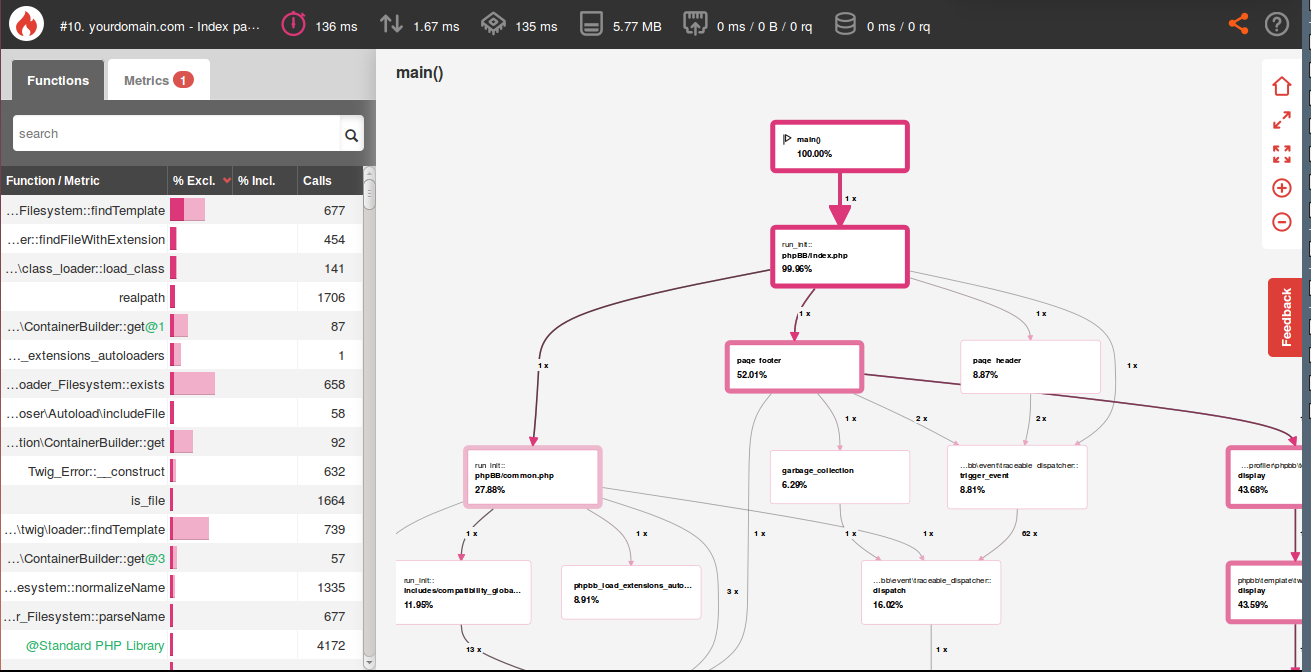
\includegraphics[width=0.8\textwidth]{images/blackfire-exemple}
  %\vspace{-22pt}
  \caption{Exemple de profil généré par \Blackfire}
  \centering
\end{center}
\end{figure}

Dernier outil développé par l'équipe produit de \emph{SensioLabs}, \Blackfire,
sorti commercialement le 27 juillet 2015 après une année de béta test publique, est un produit disponible en mode \gls{SaaS} permettant d'analyser les performances d'applications \PHP de manière simple, précise et juste.

\Blackfire fournit un moyen pour instrumenter automatiquement un code \PHP existant afin d'en extraire des données telles que le \gls{graphe d'appels} du programme ou le temps passé dans chaque fonction, et de les représenter sous une forme graphique intuitive permettant ainsi au développeur d'identifier les principaux problèmes de performance de son application.\footnote{Voir chapitre \vref{chap:Blackfire} pour plus de détails sur \Blackfire et son fonctionnement}

%	\section{Python}
% \Python est un langage de programmation 

\chapter{Objectifs}
	\setcounter{chapter}{2}
	
\begin{figure}[!h]
\begin{center}
  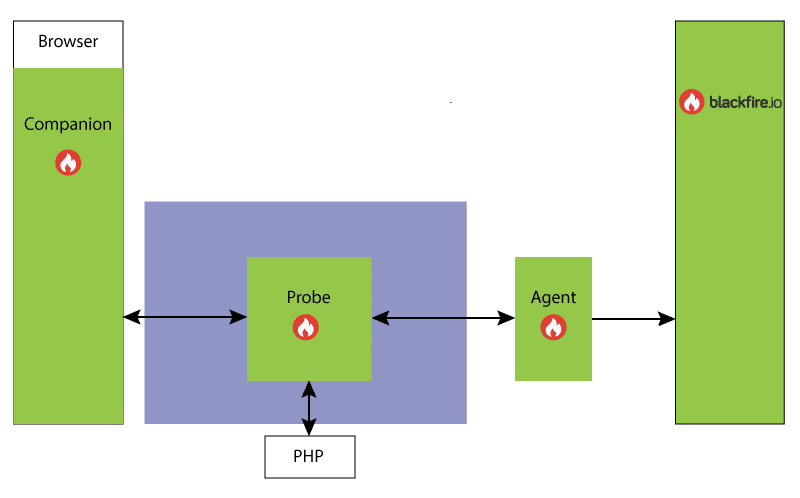
\includegraphics[width=0.8\textwidth]{images/schemas/workflow/archi-general}
  \caption{Organisation générale de \Blackfire}
  % TODO remplacé par le même schéma en simplifié (moins de flèches. le but est de montrer les composants et qui utilise quoi)
\end{center}
\end{figure}

\Blackfire est organisé en quatre composants communiquant les uns avec les autres:
\begin{itemize}
\item Le \textbf{compagnon}, disponible dans \emph{Chrome}, sert à déclencher l'analyse.
\item \textbf{blackfire.io} est le site web qui affiche les résultats.
\item L'\textbf{agent} fait le liens entre la sonde et le site blackfire.io.
\item La \textbf{sonde} est branchée sur le programme de l'utilisateur et collecte des données.
\end{itemize}

Les trois premiers composants ont été conçus de manière à être génériques, et devraient donc être capables de traiter des données issues de n'importe quelle technologie du moment que le protocole\footnote{Voir section \vref{sec:BlackfireProtocol}} est respecté. En pratique il est effectivement possible d'afficher via \textbf{blackfire.io} des profils générés via d'autres outils tel que Callgrind\footnote{\url{http://blog.blackfire.io/cli-upload.html}}, Google Chrome JavaScript CPU profiles\footnote{\url{http://blog.blackfire.io/chrome-cpu-profiles.htmll}} et bien d'autres\footnote{\url{http://blog.blackfire.io/profiling-web-page-loading-performance.html}}\footnote{\url{http://blog.blackfire.io/blackfire-file-format.html}}.

Mais le principal problème d'utiliser ces outils c'est que l'on n'a pas la même expérience que lorsqu'on profile un code \PHP avec \emph{Blackfire}. En effet, lorsqu'on n'utilise pas \Blackfire pour collecter les données on ne peut pas utiliser le compagnon pour déclencher un profil en un clic. De plus l'impact de la collecte des données sur les performances peut être important, et surtout, l'expérience utilisateur peut être compliquée : on peut être obligé d'instrumenter manuellement son code, et une fois le profil généré il faut encore le convertir dans le format utilisé par \Blackfire et l'envoyer sur le site \emph{blackfire.io} à l'aide de la commande \verb|blackfire upload|.

L'enjeu du travail effectué est multiple. Il s'agit d'une part de démontrer que la plate-forme \Blackfire est effectivement générique (et le cas échéant de corriger dans la plate-forme ou le protocole les différents problèmes qui empêchent ou gênent cette généricité), et d'autre part d'apporter le support du langage \emph{Python}.

L'objectif est donc de réaliser une nouvelle implémentation de la quatrième partie, la sonde. Celle-ci serait capable d'analyser des programmes \Python avec une expérience utilisateur la plus proche possible de celle que l'on a actuellement avec la sonde \emph{PHP}. Cela implique que la sonde doit :
\begin{itemize}
  \item permettre d'analyser du code \emph{Python}\footnote{Ceci implique à minima de collecter le graphe d'appels du programme et le temps passé dans chaque fonction/méthode}
  \item communiquer avec l'agent en respectant le protocole
  \item avoir un impact (\gls{overhead}) minimal\footnote{Afin de garantir des résultats aussi fidèles à la réalité que possible}
  \item instrumenter le code automatiquement
  \item ne déclencher l'analyse qu'à la demande\footnote{De cette manière la sonde peut être déployée en production}
\end{itemize}

\setcounter{part}{0}
\setcounter{chapter}{0} 
  
  \mainmatter
  
\fancypagestyle{plain}{%
  %\fancyhf{}
  \renewcommand{\headrulewidth}{0.5pt}
  \renewcommand{\footrulewidth}{0.5pt}
  \fancyfoot[L]{
    \logoBF[height=0.5cm]
    \logoSL[height=0.5cm]
    \logoIMAG[height=0.5cm]
  }
  \fancyfoot[R]{Page \thepage\ sur \pageref{LastPage}}
  \fancyfoot[C]{Rapport de projet de fin d'études}
}
  \pagestyle{main}

\renewcommand{\thefigure}{\thepart.\thesection-\arabic{figure}}
\renewcommand{\thesubfigure}{\thepart.\thesection-\arabic{figure}}

  %\pagestyle{fancy}

  
  % Problématique, objectifs
  % entreprise (1 page)
  % enjeu de votre PFE pour l'entreprise, position de votre équipe au sein de l'entreprise, qui vous encadre (une personne, une équipe, ...), suivi de votre travail (journée typique, ...).  
  % Faire comprendre de manière concise et intelligible par une personne non spécialiste du domaine la problématique de votre projet (~5 pages)
  %		le contexte du projet (vue d'ensemble à travers par ex. un workflow simplifié)
  %		le travail à réaliser ou le problème à résoudre
  %		les objectifs précis attendus  
  % Présentation des solutions techniques étudiées ou mises en oeuvre  (~10 pages)
  % 		synthèse de l'existant (couverture fonctionnelle existante (architecture logicielle par ex.), contraintes inhérentes au projet (outils, librairies, ...), s'appuyant sur une bibliographie précise
  % 		description de la (ou des) solution(s) envisagée(s) et des outils qui seront utilisés
  % 		protocole d'évaluation envisagé pour valider votre solution ou mesurer son efficacité
  % Votre avancement (~2 pages)
 % 		planning prévisionnel montrant ce qui a déjà été fait et ce qu’il reste à faire (présenté sous la forme d’un diagramme de Gantt)
 
  %\part{Analyse de l'existant}
    \part{Analyse de l'existant}
\thispagestyle{part}
\parttoc

	\chapter{Blackfire}
	\label{chap:Blackfire}
		\section{Architecture générale}
			% Schéma :  https://d2vqbs7xgyce6n.cloudfront.net/assets/v44abae9bcb/bundles/blackfire/img/general-workflow.png
			% Pour chaque composant : rôle/objectifs/problématiques... (Agent / Sonde / API / Companion)
			% En commentaire du schéma montrant comment ils s'organisent entre eux
	
\begin{figure}[!h]
\begin{center}
  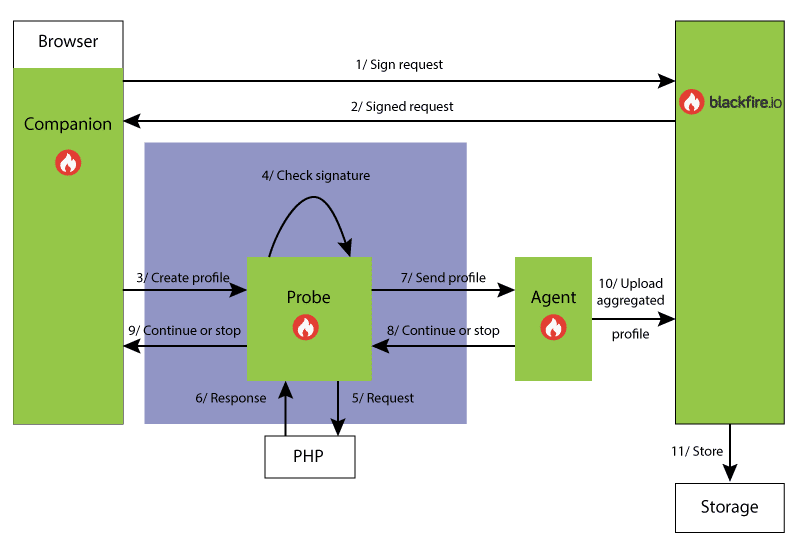
\includegraphics[width=0.8\textwidth]{images/schemas/workflow/general-workflow}
  \caption{Fonctionnement général de \Blackfire}
\end{center}
\end{figure}

Ce graphique montre comment les quatre composants de \Blackfire interagissent entre eux lors de l'établissement d'un profil.
 
Ainsi, on commence par le \textbf{Compagnon}. Son rôle est de générer la requête\footnote{Voir section \vref{subsec:BlackfireQuery}} en communiquant avec le site blackfire.io, de l'envoyer à la sonde, puis d'afficher un retour à l'utilisateur sur le statut de son profil : y a-t-il eu une erreur ? et sinon, quels sont les coûts principaux\footnote{On parle ici des temps du nœud racine, main, ou encore des coûts d'enveloppe.} ?

Ensuite, une fois que la \textbf{Sonde} a reçu la requête, celle-ci va la vérifier, instrumenter le code de l'application et analyser ce dernier. Le profil est ensuite envoyé à l'agent\footnote{Voir section \vref{subsec:comm-agent}} qui retourne un statut que la sonde retransmet au compagnon\footnote{Voir section \vref{subsec:comm-compagnon}}. Le rôle de la sonde est donc d'instrumenter le code, de générer le profil puis de l'envoyer à l'agent.

Une fois que l'\textbf{Agent} a reçu le profil, il va le vérifier et le pré-traiter, entre autres pour anonymiser certains arguments de fonction comme les requêtes SQL, qui sont susceptibles de contenir des informations sensibles. Puis il va envoyer ce profil au site blackfire.io.

Enfin, le site \textbf{blackfire.io}\footnote{Aussi appelé \textbf{API} par la suite}, a pour rôle de stocker et d'afficher les profils aux utilisateurs.

		\section{Protocole}
			\label{sec:BlackfireProtocol}
			% Retour sur certains éléments du protocole
Pour faire communiquer les différents composants entre eux, \Blackfire utilise un protocole textuel répondant à quatre objectifs principaux :
\begin{itemize}
\item Authentifier une demande de profil
\item Fournir les informations nécessaires pour générer le profil
\item Transmettre le profil généré
\item Fournir un retour à l'utilisateur
\end{itemize}

			\subsection{La Requête}
			\label{subsec:BlackfireQuery}
				% émise par le companion ou l'outil CLI via run/curl
				% pas de détail sur la signature ou le contenu précis de la requête. On se contente de ce que l'on va utiliser plus tard
La requête, émise par le client\footnote{Via l'utilisation du compagnon par exemple} permet à la fois d'authentifier une demande de profil et de fournir à la sonde un certain nombre d'options de configuration relatives au profil à générer.

Pour cela la requête est composée de deux parties:
\begin{itemize}
\item Une série d'arguments, accompagnée d'une signature cryptographique qui permet d'authentifier la demande et d'en vérifier la validité
\item Une série d'options de configuration permettant d'activer ou de désactiver certaines parties de la sonde\footnote{Par exemple l'option \verb|flag_cpu| permet de désactiver la collecte des temps CPU}.
\end{itemize}

			\subsection{Communication avec le Compagnon}
			\label{subsec:comm-compagnon}
				% Y a-t-il autre chose que le Blackfire-Response: continue ici ? Expliquer l'enjeu et l'importance de cet en-tête
L'un des usages de \Blackfire est de profiler, à l'aide du compagnon, une page web servie par un serveur distant. Dans ce cas, tout se déroule sur le serveur distant et l'utilisateur n'a aucun moyen de consulter ce qui est produit durant l'analyse. Par conséquent il est important de fournir au compagnon un retour indiquant si le profil a été généré. Cette réponse, générée par l'agent, est ensuite retransmise par la sonde au compagnon en définissant l'en-tête \verb|X-Blackfire-Response| dans la réponse \emph{HTTP}.

			\subsection{Communication avec l'agent}
			\label{subsec:comm-agent}
				% Format du hello prolog
				% La réponse de l'agent (avec les fn args)
L'analyse est déclenchée par le compagnon mais elle est réellement gérée par l'agent. Pour cela il existe un protocole en deux étapes\footnote{NB: Le protocole a évolué dans un version récente de \Blackfire avec l'introduction du fichier \verb|.blackfire.yml|} entre la sonde et l'agent.

La première étape consiste à faire authentifier la requête par l'agent\footnote{En réalité l'agent n'authentifie pas la requête mais demande à l'API de le faire} et à récupérer les dernières informations requises pour effectuer l'analyse\footnote{Les arguments de fonction si supporté}.

Pour cela la sonde commence par envoyer deux en-tête à l'agent. Le premier, \verb|Blackfire-Query| contient la partie signée de la requête (et la signature) afin que l'agent la valide. Le second, \verb|Blackfire-Probe| permet d'identifier la technologie instrumentée.

\begin{listing}[H]
\caption{En-têtes envoyés à l'agent par la sonde}
\begin{textcode}
Blackfire-Query: <requête>
Blackfire-Probe: python-20706f0
\end{textcode}
\end{listing}
Ici l'en-tête  \verb|Blackfire-Probe| indique que l'on analyse du python en version 34014960 (tel que défini par \mintinline{python}{hex(sys.hexversion)}).

La seconde partie consiste en une réponse envoyé par l'agent et contenant une ligne de statut. En cas d'erreur celle-ci est de la forme \verb|Blackfire-Error: <code> <raison>| et est destinée à être journalisée par la sonde. Sinon elle est de la forme \verb|Blackfire-Response: <message>| et est destinée à être retransmise telle quelle au compagnon. En plus du statut, l'agent peu aussi renvoyer des informations identifiant des fonctions dont on désire récupérer les arguments. Ces informations se trouvent sous la forme d'une série de lignes ayant le format suivant: \verb|Blackfire-Fn-Args: <fonction> <argument>|,
\verb|<nœud>| étant le nom de la fonction à instrumenter (tel qu'affichée dans le graphe) et \verb|<argument>| le nombre d'arguments à récupérer.

Par exemple les lignes suivantes indiquent de récupérer le premier argument de la fonction \verb|logging.error| et les deux premiers arguments de la méthode \verb|log| de la classe \verb|logging.error|
\begin{listing}[H]
\caption{En-têtes définissant les arguments de fonction à récupérer}
\begin{textcode}
Blackfire-Fn-Args: logging.error 1
Blackfire-Fn-Args: logging.Logger::log 2
\end{textcode}
\end{listing}

				\subsection{Format des profils}
					% cf: http://blog.blackfire.io/blackfire-file-format.html
\Blackfire utilise un format textuel\footnote{Voir Annexe \vref{app:fullProfile} pour un exemple complet de profil} pour décrire les profils générés après l'analyse d'un programme.

Les profils sont composés de deux sections séparées par une ligne vide. La première définit un certain nombre d'en-têtes décrivant le contexte du profil. Ainsi les principaux en-têtes sont:
\begin{itemize}
\item \verb|file-format: BlackfireProbe| qui définit le format utilisé, celui-ci ayant évolué au cours du temps\footnote{La sonde \PHP actuelle ainsi que la sonde \Python utilisent le format} \emph{BlackfireProbe}
\item \verb|graph-root-id: <nom>| définit le nom du nœud racine du graphe
\item \verb|cost-dimensions: <liste>| définit la liste des dimensions envoyées par la sonde (temps \emph{wall-time}, cpu, consommation mémoire...). Les dimensions sont séparées par des espaces
\item \verb|probed-os: <os>|, \verb|probed-language: <laguage>|, \verb|probed-version: <language version>| permet de définir l'environnement d'exécution du programme.
\end{itemize}

La seconde section définit le graphe à proprement parler. Celui-ci est construit à partir de ses arcs, ne ligne correspondant à un arc.

\begin{listing}[H]
\caption{Ligne de profil simple (pas d'argument de fonction)}
\begin{textcode}
<appelant>==><appelé>//<coûts>
\end{textcode}
\end{listing}

\begin{itemize}
\item \verb|<appelant>| est le nom du nœud appelant
\item \verb|<appelé>| est le nom du nœud appelé
\item \verb|<coûts>| est la liste des coûts pour le lien. Les coûts sont séparés par des espaces et correspondent aux dimensions définies précédemment.
\end{itemize}

	\chapter[Analyse en \Python]{Analyse de performances en \Python}
Il existe différents outils et API permettant d'analyser les performances ou le comportement d'un code \Python et on peut regrouper ces outils en deux catégories : ceux qui fonctionnent en mode \gls{SaaS} (comme \Blackfire) et ceux qui fonctionnent de manière indépendante ou sont directement intégrés dans \Python.

		\section{Outils tiers existants}
Il existe plusieurs outils tiers permettant de s'intéresser au fonctionnent d'une application \Python et parmi ceux-là l'un d'entre eux va nous occuper : \emph{New Relic\footnote{\url{https://www.newrelic.com}}}. %et \emph{Opbeat\footnote{\url{https://www.opbeat.com}}}.

			\subsection{New Relic}
          		\begin{wrapfigure}{r}{0.5\textwidth}
  \vspace{-30pt}
  \begin{center}
    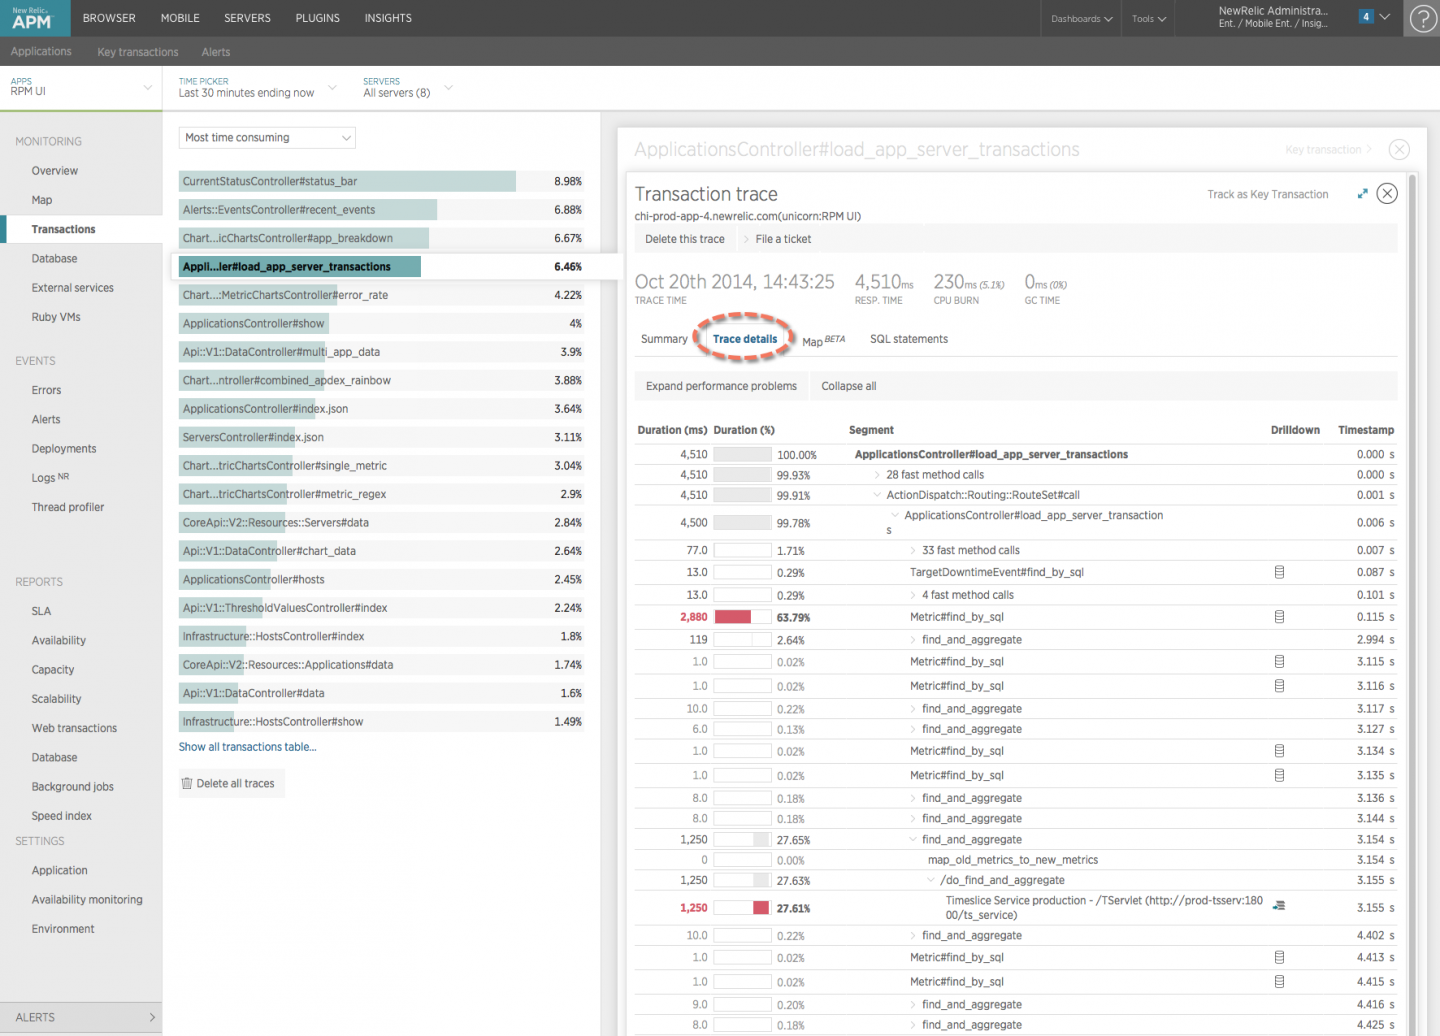
\includegraphics[width=0.48\textwidth]{images/new-relic_trace}
  \end{center}
  \vspace{-22pt}
  \caption{\emph{New Relic} - exemple de trace}
  \vspace{-20pt}
\end{wrapfigure}

\emph{New Relic} est un outil disponible en mode \gls{SaaS} permettant de monitorer les serveur de \gls{production} tout en ayant un impact sur les performances négligeable.

Ils proposent différentes fonctionnalités dont notamment une permettant d'afficher, sous forme de trace, des métriques sur le code exécuté. Il va ainsi permettre d'afficher une trace, un profil du code exécuté avec le temps passé dans chaque fonction.
 
\clearpage
Cet outil est intéressant sur plusieurs points :
\begin{itemize}
  \item Le langage \Python est supporté
  \item L'expérience utilisateur est proche de celle de \Blackfire (pas ou peu d'instrumentation manuelle de requise)
\end{itemize}
  
Enfin le code source du module de l'agent \emph{New Relic} pour \Python est disponible sur \gls{PyPI}\footnote{\url{https://pypi.python.org/pypi/newrelic}} ce qui permet de comprendre son fonctionnement.
  
  \subsubsection{Collecte des métriques}
Pour collecter le graphe d'appels et les temps associés deux techniques semblent être en œuvre :
Tout d'abord l'agent va lancer un thread spécial qui sera chargé de récupérer la \gls{pile d'appels} à intervalle régulier et de l'utiliser pour reconstituer le \gls{graphe d'appels} du programme.
 
En parallèle diverses méthodes et fonctions estimées importantes sont décorés afin de récupérer plus d'information comme le temps d'exécution ou la requête SQL exécutée.

Cette instrumentation se fait en plusieurs étapes \footnote{Voir Annexe \vref{app:newrelicdecorationmethodes} pour le code correspondant} :
\begin{enumerate}
  \item Définition d'un \emph{\gls{chargeur de module}} personnalisé afin de décorer automatiquement les modules quand ils sont chargés.
  \item Lecture dans le fichier de configuration de la liste des méthodes à décorer.
  \item Enregistrement d'un \emph{\gls{hook}} pour chacune des méthode à décorer auprès du chargeur de module.
  \item Lors du chargement d'un module, le chargeur de module va exécuter tous les hooks se rapportant au module en question afin d'en décorer les méthodes.
\end{enumerate}

Cette instrumentation fonctionne à partir d'un fichier de configuration indiquant quelles méthodes doivent être instrumentées, elle est donc parfaitement générique. En outre le fait de n'instrumenter qu'une partie des appels de fonctions permet de l'imiter l'impact du profileur au point d'en être négligeable, surtout qu'il existe une librairie\footnote{\url{https://pypi.python.org/pypi/wrapt}} (écrite dans le langage C) permettant de décorer facilement et à moindre coup n'importe quelle fonction ou méthode \Python.

En revanche cette technique impose de connaître et d'indiquer à l'avance la liste exhaustive des fonctions intéressantes.

  \subsubsection{Expérience utilisateur}
			%\subsection{Optbeat}
			%	  \subsubsection{Présentation}
  \subsubsection{Fonctionnalités}
  \subsubsection{Fonctionnement}
			
		\section{Python}
			%\subsection{Pycallgraph}
			%\label{subsec:pycallgraph}
			%	\input{existant/python-python-pycallgraph} 
			%\subsection{Pyinstrument}
			%\label{subsec:pyinstrument}
			%	\input{existant/python-python-pyinstrument}
			\subsection{Python C-Profiler / \textunderscore lsprof} 
			\label{subsec:cprofiler}
				\Python fournit trois modules\footnote{\url{https://docs.python.org/2/library/profile.html}} permettant d'analyser les performances d'un programme et de générer des rapports à partir des données collectées. Ils utilisent tous les trois la même technique, à savoir l'utilisation de \verb|sys.setprofile()|\footnote{\verb?sys.setprofile()? ayant la particularité d'être intégré directement dans le cœur de \Python et d'accepter n'importe quelle fonction de rappel, qu'elle soit écrite en \C ou en \Python - Voir \url{https://docs.python.org/2/library/sys.html#sys.setprofile} pour plus de détails} pour définir une fonction de rappel qui est appelée à chaque fois que l'interpréteur entre ou sort d'une fonction. L'événement \verb|CALL|\footnote{Lancé quand l'interpréteur entre dans une fonction} permettant de récupérer le nom de la fonction et de relever la date\footnote{La date est relevée de la manière la plus précise possible, la résolution restant néanmoins dépendante du système sur lequel l'application tourne} lorsque celle-ci au début de la fonction, et l'événement \verb|RETURN|\footnote{Lancé quand l'interpréteur sort d'une fonction} permettant de mesurer la date en sortie de la fonction, de calculer la différence entre le début et la fin de cette dernière et de stocker le résultat.

De plus ces trois modules collectent les mêmes données, à savoir les temps exclusif\footnote{En excluant le temps passé dans les autres fonctions} et inclusif\footnote{En incluant le temps passé dans les autres fonctions} passés dans chaque fonction et le nombre de fois qu'elle a été appelée. De plus ils génèrent leur rapport dans le même format, à savoir \verb|pstat|\footnote{\url{https://docs.python.org/2/library/profile.html#module-pstats}}, mais ils ont néanmoins de grandes différences d'implémentation et ne servent pas le même usage : 

\begin{itemize}
\item \textbf{cProfile} est le module recommandé dans la majorité des cas, il s'agit d'une extension \C ayant un impact sur les performances relativement limité.
\item \textbf{profile} est un module écrit en pur \Python et ayant exactement la même interface que le \emph{cProfile}. Par contre son impact sur les performances est très important, mais étant écrit en \Python il est plus facile de le modifier et de l'étendre.
\item \textbf{hotshot} est un autre module écrit en \C. A la différence du \emph{cProfile} son objectif est d'avoir un impact sur les performances le plus faible possible, quitte à devoir passer plus de temps dans une phase de post-traitement. En revanche il n'est plus maintenu aujourd'hui et a été supprimé dans \Python 3.
\end{itemize}
			\subsection{Yappi}
			\label{subsec:yappi}
				\emph{Yappi}\footnote{\url{https://bitbucket.org/sumerc/yappi}}, pour \emph{Yet Another Python Profiler}, est un logiciel open source\footnote{Sous licence \emph{MIT}} créé en 2009 par \emph{Sümer Cip} et permettant d'analyser les performances d'un programme \emph{Python}.

Il s'agit d'un module écrit en \C utilisant le même fonctionnement que le \emph{C-Profiler}, dont il est inspiré (à savoir l'utilisation d'une fonction de rappel qui est appelée à chaque fois que l'on entre ou sort d'une fonction).

D'un point de vue fonctionnel, \emph{Yappi} a été conçu de manière à avoir un impact sur les performances de l'application mesurée le plus faible possible, et dispose de quelques fonctionnalités qui ne sont pas présentes dans le \emph{C-Profiler} :
\begin{itemize}
\item Possibilité d'avoir des temps CPU à la place des temps utilisateur
\item Gestion du multi threading
\begin{itemize}
\item Les threads sont automatiquement analysés
\item Les appels de fonction des différents threads ne sont pas différenciés (on ne peut pas savoir quel thread a effectué un appel de fonction donné) 
\item Le temps total passé dans chaque thread est disponible
\end{itemize}
\end{itemize}
				
				
				
				
				
				
				
				
				
				
				
				
				
				
				
				
				
				
				
				
				
				
				
				
				
				
				
				
				
				
				
				
				 
    %\chapter{Blackfire}
      %\chapter{Blackfire}
      %\section{Sonde}
       % \section{Sonde}
      %\section{Agent}
        %\section{Agent}
      %\section{API}
        %\section{API}
    %\chapter{Analyse de performance en Python}
      %\chapter{Analyse de performance en \Python}
Il existe différents outils et API permettant d'analyser les performances ou le comportement d'un code python et on peut regrouper ses outils en 2 catégories : ceux qui fonctionnent en mode \gls{SaaS} (comme \Blackfire) et ceux qui fonctionnent de manière indépendante où sont directement intégré dans \Python.
      %\section{Outils tiers existants}
       % \section{Outils tiers existants}
Il existe plusieurs outils tiers permettant de s'intéresser au fonctionnent d'une application \Python et parmi ceux là deux vont nous occuper : \emph{New Relic\footnote{https://www.newrelic.com}} et \emph{Opbeat\footnote{https://www.opbeat.com}}.
        %\subsection{New Relic}
         % \begin{wrapfigure}{r}{0.5\textwidth}
  \vspace{-30pt}
  \begin{center}
    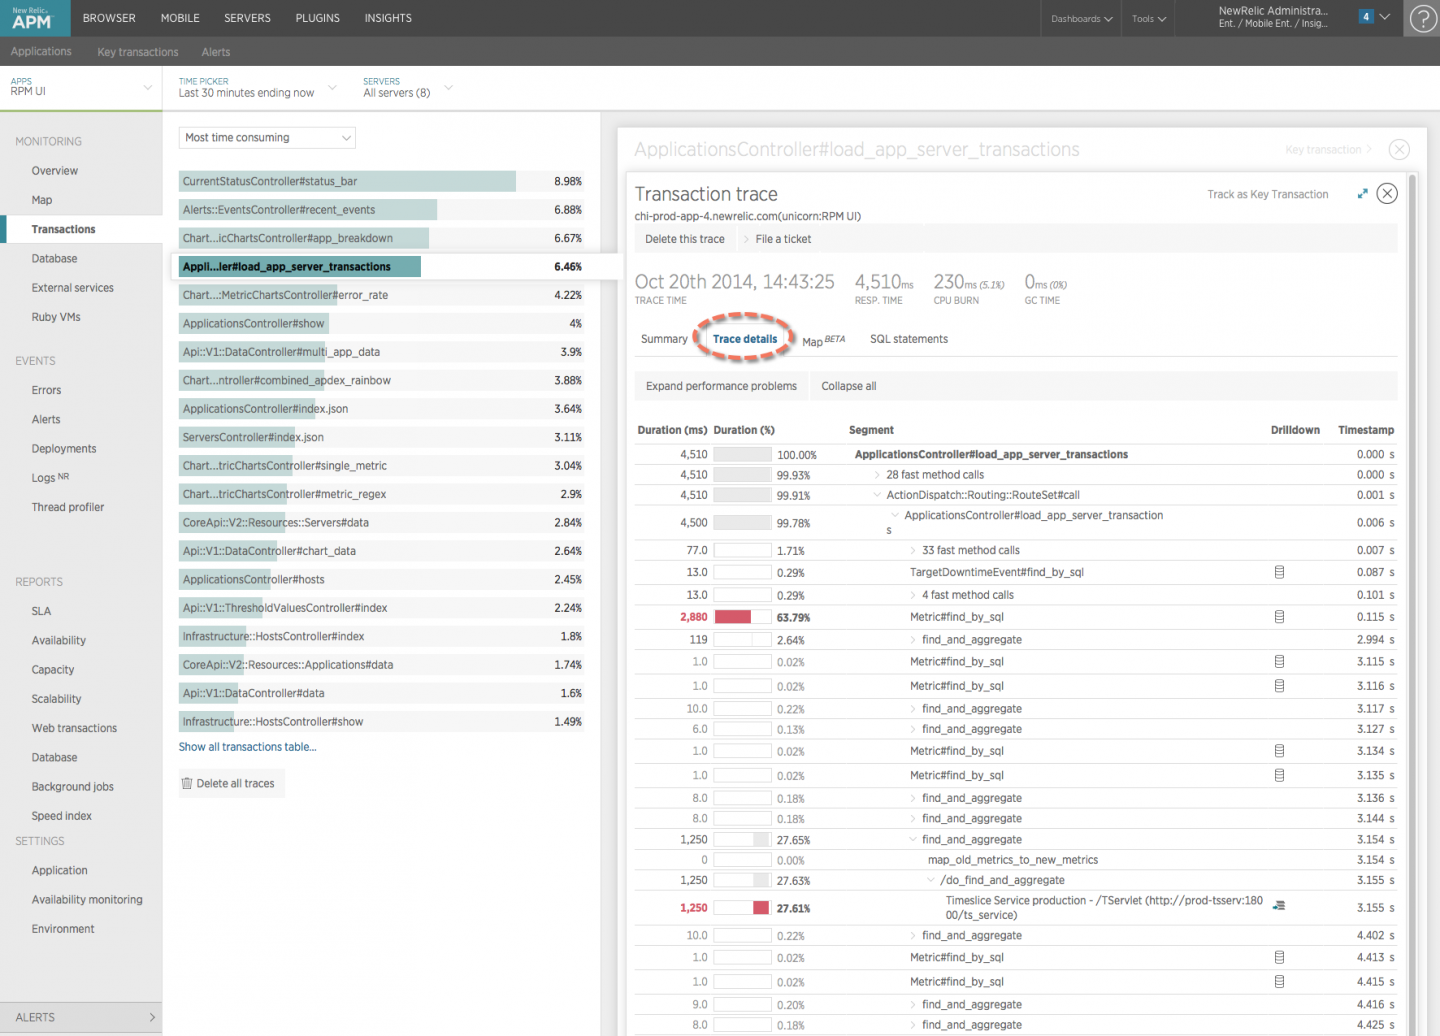
\includegraphics[width=0.48\textwidth]{images/new-relic_trace}
  \end{center}
  \vspace{-22pt}
  \caption{\emph{New Relic} - exemple de trace}
  \vspace{-20pt}
\end{wrapfigure}

\emph{New Relic} est un outil disponible en mode \gls{SaaS} permettant de monitorer les serveur de \gls{production} tout en ayant un impact sur les performances négligeable.

Ils proposent différentes fonctionnalités dont notamment une permettant d'afficher, sous forme de trace, des métriques sur le code exécuté. Il va ainsi permettre d'afficher une trace, un profil du code exécuté avec le temps passé dans chaque fonction.
 
\clearpage
Cet outil est intéressant sur plusieurs points :
\begin{itemize}
  \item Le langage \Python est supporté
  \item L'expérience utilisateur est proche de celle de \Blackfire (pas ou peu d'instrumentation manuelle de requise)
\end{itemize}
  
Enfin le code source du module de l'agent \emph{New Relic} pour \Python est disponible sur \gls{PyPI}\footnote{\url{https://pypi.python.org/pypi/newrelic}} ce qui permet de comprendre son fonctionnement.
  
  \subsubsection{Collecte des métriques}
Pour collecter le graphe d'appels et les temps associés deux techniques semblent être en œuvre :
Tout d'abord l'agent va lancer un thread spécial qui sera chargé de récupérer la \gls{pile d'appels} à intervalle régulier et de l'utiliser pour reconstituer le \gls{graphe d'appels} du programme.
 
En parallèle diverses méthodes et fonctions estimées importantes sont décorés afin de récupérer plus d'information comme le temps d'exécution ou la requête SQL exécutée.

Cette instrumentation se fait en plusieurs étapes \footnote{Voir Annexe \vref{app:newrelicdecorationmethodes} pour le code correspondant} :
\begin{enumerate}
  \item Définition d'un \emph{\gls{chargeur de module}} personnalisé afin de décorer automatiquement les modules quand ils sont chargés.
  \item Lecture dans le fichier de configuration de la liste des méthodes à décorer.
  \item Enregistrement d'un \emph{\gls{hook}} pour chacune des méthode à décorer auprès du chargeur de module.
  \item Lors du chargement d'un module, le chargeur de module va exécuter tous les hooks se rapportant au module en question afin d'en décorer les méthodes.
\end{enumerate}

Cette instrumentation fonctionne à partir d'un fichier de configuration indiquant quelles méthodes doivent être instrumentées, elle est donc parfaitement générique. En outre le fait de n'instrumenter qu'une partie des appels de fonctions permet de l'imiter l'impact du profileur au point d'en être négligeable, surtout qu'il existe une librairie\footnote{\url{https://pypi.python.org/pypi/wrapt}} (écrite dans le langage C) permettant de décorer facilement et à moindre coup n'importe quelle fonction ou méthode \Python.

En revanche cette technique impose de connaître et d'indiquer à l'avance la liste exhaustive des fonctions intéressantes.

  \subsubsection{Expérience utilisateur}
          %\subsubsection{Présentation}
          %\subsubsection{Fonctionnalités}
          %\subsubsection{Fonctionnement}
        %\subsection{Optbeat}
        %    \subsubsection{Présentation}
  \subsubsection{Fonctionnalités}
  \subsubsection{Fonctionnement}
          %\subsubsection{Présentation}
          %\subsubsection{Fonctionnalités}
          %\subsubsection{Fonctionnement}
      %\section{Python}
      %  \input{existant/python-python}
        %\subsection{Pycallgraph}
       %   \input{existant/python-python-pycallgraph}
        %\subsection{Pyinstrument}
       %   \input{existant/python-python-pyinstrument}
        %\subsection{Python C-Profiler/_lsprof}
       %   \Python fournit trois modules\footnote{\url{https://docs.python.org/2/library/profile.html}} permettant d'analyser les performances d'un programme et de générer des rapports à partir des données collectées. Ils utilisent tous les trois la même technique, à savoir l'utilisation de \verb|sys.setprofile()|\footnote{\verb?sys.setprofile()? ayant la particularité d'être intégré directement dans le cœur de \Python et d'accepter n'importe quelle fonction de rappel, qu'elle soit écrite en \C ou en \Python - Voir \url{https://docs.python.org/2/library/sys.html#sys.setprofile} pour plus de détails} pour définir une fonction de rappel qui est appelée à chaque fois que l'interpréteur entre ou sort d'une fonction. L'événement \verb|CALL|\footnote{Lancé quand l'interpréteur entre dans une fonction} permettant de récupérer le nom de la fonction et de relever la date\footnote{La date est relevée de la manière la plus précise possible, la résolution restant néanmoins dépendante du système sur lequel l'application tourne} lorsque celle-ci au début de la fonction, et l'événement \verb|RETURN|\footnote{Lancé quand l'interpréteur sort d'une fonction} permettant de mesurer la date en sortie de la fonction, de calculer la différence entre le début et la fin de cette dernière et de stocker le résultat.

De plus ces trois modules collectent les mêmes données, à savoir les temps exclusif\footnote{En excluant le temps passé dans les autres fonctions} et inclusif\footnote{En incluant le temps passé dans les autres fonctions} passés dans chaque fonction et le nombre de fois qu'elle a été appelée. De plus ils génèrent leur rapport dans le même format, à savoir \verb|pstat|\footnote{\url{https://docs.python.org/2/library/profile.html#module-pstats}}, mais ils ont néanmoins de grandes différences d'implémentation et ne servent pas le même usage : 

\begin{itemize}
\item \textbf{cProfile} est le module recommandé dans la majorité des cas, il s'agit d'une extension \C ayant un impact sur les performances relativement limité.
\item \textbf{profile} est un module écrit en pur \Python et ayant exactement la même interface que le \emph{cProfile}. Par contre son impact sur les performances est très important, mais étant écrit en \Python il est plus facile de le modifier et de l'étendre.
\item \textbf{hotshot} est un autre module écrit en \C. A la différence du \emph{cProfile} son objectif est d'avoir un impact sur les performances le plus faible possible, quitte à devoir passer plus de temps dans une phase de post-traitement. En revanche il n'est plus maintenu aujourd'hui et a été supprimé dans \Python 3.
\end{itemize}
        %\subsection{Yappi}
      %    \emph{Yappi}\footnote{\url{https://bitbucket.org/sumerc/yappi}}, pour \emph{Yet Another Python Profiler}, est un logiciel open source\footnote{Sous licence \emph{MIT}} créé en 2009 par \emph{Sümer Cip} et permettant d'analyser les performances d'un programme \emph{Python}.

Il s'agit d'un module écrit en \C utilisant le même fonctionnement que le \emph{C-Profiler}, dont il est inspiré (à savoir l'utilisation d'une fonction de rappel qui est appelée à chaque fois que l'on entre ou sort d'une fonction).

D'un point de vue fonctionnel, \emph{Yappi} a été conçu de manière à avoir un impact sur les performances de l'application mesurée le plus faible possible, et dispose de quelques fonctionnalités qui ne sont pas présentes dans le \emph{C-Profiler} :
\begin{itemize}
\item Possibilité d'avoir des temps CPU à la place des temps utilisateur
\item Gestion du multi threading
\begin{itemize}
\item Les threads sont automatiquement analysés
\item Les appels de fonction des différents threads ne sont pas différenciés (on ne peut pas savoir quel thread a effectué un appel de fonction donné) 
\item Le temps total passé dans chaque thread est disponible
\end{itemize}
\end{itemize}
        %\subsection{WSGI middle-ware}
       %   \input{existant/python-python-wsgi}
  %\part{Implémentation}
    \part{Implémentation}
\thispagestyle{part}
\parttoc
%\thispagestyle{part}
 
  %\chapter{Considérations générales}
  %\section{Objectifs}
  %Pour rappel, l'objectif est de fournir une sonde ayant répondant à un certain nombre de critères:
  %\begin{itemize}
  %  \item Elle doit permettre d'analyser du code \Python
  %  \item Elle doit communiquer avec l'\gls{agent} en utilisant un protocole propre à \Blackfire
  %  \item Elle doit générer le \gls{graphe d'appels} du programme
  %  \item Elle doit collecter des métriques sur le temps passé dans chaque fonction/méthode
  %  \item L'\gls{overhead} induit par la sonde doit être minimal
  %  \item L'instrumentation du code doit être automatique
  %  \item Conformément au protocole, la sonde ne doit déclencher l'analyse que à la demande
  %\end{itemize}

%  \section{Travail effectué}
%  Le travail effectué a donné lieu à deux implémentations de la sonde. Une première écrite uniquement en Python servant essentiellement de preuve de faisabilité et ayant certains problèmes de performance. Et une seconde reprenant le travail effectué sur la première implémentation mais avec les parties critiques, d'un point de vue performances, écrites directement en \C.
  
La sonde est découpée en trois grandes parties : trois modules correspondant aux trois rôles principaux de la sonde, à savoir :
\begin{itemize}
\item \textbf{Instrumentation} \emph{automatique} : le module \mintinline{python}{blackfire} définit l'interface publique qui sera exposée à l'utilisateur, à savoir les différents points d'entrée permettant de lancer l'analyse du code.
\item \textbf{Intégration} \emph{avec Blackfire} : le module \mintinline{python}{blackfire.probe} définit la classe \\\mintinline{python}{BlackfireProbe} qui implémente le protocole utilisé pour communiquer avec l'agent \Blackfire. Cette classe est instanciée par les différents points d'entrée en un objet qui représente ainsi la sonde actuellement utilisée. La classe \mintinline{python}{BlackfireProbe} définie aussi une interface qui permet au développeur, si l'objet est exposé, de contrôler plus finement les parties du code qui sont analysées.
\item \textbf{Collecte} \emph{des données} : le module \mintinline{python}{blackfire.profiler} définit la classe \mintinline{python}{Profiler} qui est en charge de collecter les données qui formeront le profil (\gls{métriques} et \gls{graphe d'appels}).
\end{itemize}

\begin{note}[Python 3]
\Python 3 a apporté de grands changements au langage avec, par exemple, un support par défaut de l'UTF-8, mais a au passage cassé la rétro-compatibilité avec \Python 2. Cette cassure étant très importante\footnote{Voir annexe \vref{app:compat-py3} pour plus de détails}, le taux d'adoption de \Python 3 est assez faible mais en constante progression. Il est donc important pour \Blackfire de supporter les deux versions.
\end{note}
% TODO note sur cPython vs Pypy and others

  \chapter[Instrumentation]{Instrumentation automatique}
\Blackfire est un outil destiné à être utilisé aussi bien lors du développement que sur des sites en production. Cela implique que, même si l'\gls{overhead} induit par la sonde est très faible, la sonde ne doit être activée que si un profil a été demandé afin d'éviter de générer des milliers (voir des millions) de profils inutilement.

Cette partie a donc pour rôle de s'assurer qu'un profil a été demandé et ensuite de brancher dans le \gls{code utilisateur} la partie qui s'occupe de l'intégration avec le reste de l'outil. Néanmoins cette tâche doit être exécutée de manière automatique ou alors avec le minimum de modification dans le code utilisateur.

Pour cela trois principaux cas de figures sont à considérer :
\begin{itemize}
\item L'instrumentation automatique d'un programme en ligne de commande (\gls{CLI})
\item L'instrumentation automatique d'une application \gls{WSGI} (application web)
\item L'instrumentation manuelle par le développeur
\end{itemize}

\section[Programme CLI]{Instrumentation automatique d'un programme CLI}
\label{sec:instru-pythonpath}
On considère ici un programme analysé via l'utilisation de l'outil en ligne de commande. Dans ce cas il est possible d'utiliser le module \verb|site|\footnote{\url{https://docs.python.org/2/library/site.html}} de \Python afin d'instrumenter le programme automatiquement, et ceci sans aucune modification.

Cela est possible grâce au comportement particulier du module \verb|site|. En effet, il s'agit d'un module qui est importé (et donc exécuté) automatiquement lors du lancement d'un programme \Python, et l'un des rôles de ce module est de rechercher un module nommé \verb|sitecustomize| dans les différents dossiers référencés dans la variable d'environnement \verb|PYTHONPATH|\footnote{La variable d'environnement \verb?PYTHONPATH? est vide par défaut} et de l'exécuter.

\begin{listing}[H]
\caption{Exemple d'analyse d'un programme en ligne de commande}
\begin{bashcode}
 $ $ PYTHONPATH='/chemin/vers/blackfire/bootstrap/sitecustomize.py' blackfire run python mon-programme.py
\end{bashcode}
\end{listing}

Le module \verb|sitecustomize| est très simple : il regarde si la variable d'environnement \verb|BLACKFIRE_QUERY| est présente\footnote{La variable d'environnement est définie lors de l'utilisation de la commande \verb|blackfire run|, son contenu sera précisé plus tard - voir section \vref{subsec:BlackfireQuery}} et, si c'est le cas, branche \Blackfire en passant la main à la sonde à proprement parler \footnote{Voir chapitre \vref{chap:integration}}.

\begin{listing}[H]
\caption{Instrumentation automatique d'un programme en ligne de commande}
\pythonfile{codes/probe/blackfire/bootstrap/sitecustomize.py}
\end{listing}

\begin{note}
À l'avenir, on peut imaginer que l'outil en ligne de commande \Blackfire va configurer automatiquement la variable d'environnement \verb|PYTHONPATH| de l'utilisateur, ce qui permettrait de simplifier la commande précédente.
\end{note}

\section[Application WSGI]{Instrumentation automatique d'une application WSGI}
On considère ici une application web utilisant la spécification WSGI\footnote{\url{https://docs.python.org/2/library/wsgiref.html}}. Dans ce cas il est nécessaire de décorer le point d'entrée\footnote{Il s'agit de l'objet (function ou variable) qui a le nom \verb|application| dans le contexte du module renseigné auprès du serveur WSGI} de l'application par un middleware WSGI qui va se charger de vérifier la présence de l'en-tête \verb|X-Blackfire-Query|\footnoe{Cet en-tête est défini lorsque le compagnon ou la commande \verb|blackfire curl| est utilisé - voir section \vref{subsec:BlackfireQuery})} et d'activer \Blackfire le cas échéant. Ce middleware a aussi la charge de récupérer le code HTTP de la réponse (requis par le protocole) et de définir la \emph{Response Line} qui est envoyée au compagnon.

Ce middleware a été implémenté dans la classe \verb|blackfire.WSGI_wrapper|, et le décorateur \verb|blackfire.wsgi_application| permet d'en simplifier l'utilisation lorsque que le point d'entrée est une fonction\footnote{Voir Annexe \vref{app:decorateurwsgi} pour le code du décorateur}.

\begin{listing}[H]
\caption{Exemple d'utilisation du décorateur WSGI}
\pythonfile{codes/probe/test_wsgi.py}
\end{listing}

%\section{Instrumentation manuelle}

% TODO Conserver cette section ? si oui la rédiger

%\begin{listing}[H]
%\caption{Instrumentation effective du code}
%\pythonfile[firstline=9]{codes/probe/blackfire/config.py}
%\end{listing}

  \chapter[Intégration]{Intégration avec Blackfire}
  \label{chap:integration}
% Schéma pour montrer où on se situe dans l'archi/workflow ?
La sonde travaille en tandem avec l'agent, : quand la première collecte les données, le second les traite et les envoie à l'API. Ce ci implique qu'ils communiquer l'un avec l'autre, ce qu'ils font au travers d'un protocole dédié\footnote{Voir section \vref{sec:BlackfireProtocol}}.


%	\section{Protocole}
% Schéma de l'architecture/protocole complet tout en gris excepté la partie qui nous concerne
%	\subsection{La requête}
%    \label{subsec:BlackfireQuery}
  
  \chapter[Collecte]{Collecte des données}
Le rôle principal de la sonde, avant de s'intégrer avec le reste de \Blackfire, est de collecter des données, des métriques sur le code.

La sonde étant exécutée en même temps que le code utilisateur ses performances sont cruciales. Il est donc important de minimiser son impact, aussi bien sur les performances (les temps) que sur la consommation mémoire. Pour cette raison il a été décidé de l'implémenter en \C\footnote{Une première version a été implémentée en \Python afin de servir de preuve de faisabilité, et l'impact était très important ; le temps d'exécution était souvent doublé, parfois même décuplé.}.

  \section{Fonctionnement général}
La méthode utilisée pour instrumenter le code \Python est la même que celle utilisée par \emph{Yappi}\footnote{Voir section \vref{subsec:yappi}}, dont sont issus ou inspirés certains éléments de l'implémentation actuelle. À savoir l'utilisation de la méthode \verb|sys.setprofiler()| qui permet de définir une fonction de rappel appelée à chaque fois que l'interpréteur entre ou sort d'une fonction.

Dans l'implémentation actuelle, la fonction \C \verb|_blackfire_callback| est enregistrée en tant que fonction de rappel et est donc appelée à chaque fois que l'un des événements\footnote{Les événements sont toujours déclenchés avant l'exécution du code par l'interpréteur} suivants intervient :
\begin{itemize}
\item \verb|PyTrace_CALL| : exécution d'une fonction écrite en \Python
\item \verb|PyTrace_RETURN| : fin d'une fonction \Python
\item \verb|PyTrace_EXCEPTION| : fin d'une fonction \Python avec exception
\item \verb|PyTrace_C_CALL| : exécution d'une fonction écrite en \C
\item \verb|PyTrace_C_RETURN| : fin d'une fonction \C
\item \verb|PyTrace_C_EXCEPTION| : fin d'une fonction \C avec exception
\end{itemize}

Le rôle de cette fonction de rappel est double. D'un côté c'est elle qui va lancer l'analyse des différents événements, et c'est donc à partir d'elle que tout le travail de collecte de données va être effectué. De l'autre elle s'assure que les exceptions lancées par le code utilisateur sont conservées et ne sont pas écrasées si des problèmes surviennent pendant le traitement de l'événement en question\footnote{L'action de \Blackfire doit impacter aussi peu que possible le code utilisateur et cela concerne aussi la gestion des erreurs : la sonde doit être capable, autant que possible, de traiter ses propres erreurs}.

Il y a quelques différences de traitement entre les appels \C et les appels \Python car certaines données ne sont pas collectées de la même manière mais sinon le fonctionnement général est identique. De même, aucune différence n'est faite entre les fins de fonction avec et sans exception. Ainsi les six événements précédents sont répartis en deux groupes : \emph{Début} et \emph{Fin} de fonction.

L'idée est donc d'utiliser ces événements pour maintenir la \gls{pile d'appels} du programme et remplir le \gls{graphe d'appels} au fur et à mesure avec les métriques correspondantes.

  \section{Gestion du graphe d'appels}
  \label{sec:gestion-graph-appels}
La \gls{pile d'appels} du programme est construite à l'aide de l'objet \verb|frame|\footnote{Cet objet représente le contexte d'exécution de la fonction et contient donc toutes les informations sur le code exécuté. Pour plus de détails : \url{https://docs.python.org/2/library/inspect.html}} envoyé à la fonction de rappel. À chaque événement de type \emph{entrée de fonction} on identifie l'appel de fonction et on l'ajoute dans la pile.
  
Cet appel est identifié\footnote{Voir annexe \vref{app:pile_struct} pour les structures de données} par ses arguments si ceux-ci sont collectés\footnote{Voir section \vref{sec:fnargs}} et par la méthode qui est appelée, elle-même identifiée par son module, sa classe et son nom. 

À cet appel de fonction on associe ensuite une série de métriques qui reflètent l'état du système au moment où la fonction est appelée. Ainsi sont mesurés à ce moment la date en microsecondes, le temps système écoulé ou encore le nombre d'opcodes exécutés depuis le début du programme.

\begin{note}[Importation de la pile courante]
Lors de l'appel à \verb|start|, la pile d'exécution courante est importée afin de tout le temps avoir des couples appelant/appelé corrects et d'éviter de se retrouver avec des appels de fonctions orphelins (sans appelant). Pour cela on parcourt la pile courante en sens inverse (donc en partant du contexte le plus ancien) et on simule une entrée de fonction pour chaque contexte.
\end{note}

\begin{note}[Gestion des appels récursifs]
Afin d'éviter de générer des graphes cycliques\footnote{C'est à dire un graphe où les appels récursifs génèrent des cycles}, un appel de fonction est aussi identifié par son niveau de récursivité. Celui-ci correspond au nombre de fois où la fonction appelée est déjà présente dans la pile. S'il est différent de 1 il sera ajouté au nom de la fonction dans le graphe sous la forme \verb|@<niv. rec.>|.
\end{note}

\begin{note}[Performances]
Afin de contrôler l'utilisation de la mémoire\footnote{Voir section \vref{sec:performances} pour plus de détails sur la gestion des performances}, éviter que celle-ci augmente indéfiniment lors de l'analyse d'un gros programme et épargner quelques calculs, les méthodes ne sont identifiées qu'une seule fois puis mises en cache dans une table de hachage afin d'être réutilisées.
\end{note}

\subsection{Identification de la méthode appelée - Appel Python}
\label{ident-python}
Lors d'un appel \Python (appel d'une fonction écrite en \Python) le \emph{\gls{contexte d'exécution}} envoyé à la fonction de rappel correspond à celui de la fonction qui va être exécutée.

\paragraph*{Le module} Lors d'un appel \Python, le nom du module n'est pas transmis. En revanche,  via la variable \verb|frame->f_code->co_filename|, on dispose du nom du fichier contenant le code exécuté à partir duquel on peut retrouver le nom du module. Par contre il s'agit d'une opération coûteuse car elle peut impliquer de nombreux calculs et appels au système de fichiers. Mais lors d'une définition en \Python il y a une relation forte entre le module et le fichier qui le définit\footnote{Un fichier correspond toujours à un seul et unique module qui est lui même entièrement défini dans le-dit fichier} et on peut donc s'en servir à la place du nom du module (quitte à résoudre son nom plus tard si nécessaire).

\paragraph*{La classe} L'un des éléments qui différencient une fonction d'une méthode est que une méthode prend explicitement une instance de la classe en premier argument et que par convention elle s'appelle \verb|self|. Pour récupérer le nom de la classe on peut donc vérifier si le premier élément s'appelle \verb|self| et s'il est une instance d'une classe, auquel cas l'objet dispose d'un attribut \verb|__class__| contenant un objet décrivant la classe, lui même disposant d'un attribut \verb|__name__| indiquant son nom.

\paragraph*{La méthode} Le nom de la méthode est indiqué via la variable \verb|frame->f_code->co_name|.

\subsection{Identification de la méthode appelée - Appel C}
À la différence des appels \Python, lors d'un appel \C (appel d'une fonction écrite en \C depuis un code \Python) le \emph{\gls{contexte d'exécution}} envoyé à la fonction de rappel ne correspond pas à celui de la fonction qui va être exécuté mais à celui de la fonction qui vient d'être exécutée, car s'agissant d'un appel \C le travail n'est pas effectué par l'interpréteur et aucune \verb|frame| n'est générée. En revanche un object décrivant la fonction \C à exécuter\footnote{Il s'agit d'un \verb|PyCFunctionObject*|, voir annexe \vref{app:PyCFunctionObject}} est passé à la fonction de rappel en plus de l'objet \verb|frame|

\paragraph*{Le module} Lors d'un appel C le nom du module auquel la fonction est rattaché est passé via la variable \verb|function->m_module| mais plusieurs deux cas de figures sont à considérer : 
\begin{itemize}
\item La fonction fait partie des builtin\footnote{Certaines fonctions sont toujours disponibles et ne sont rattachés à aucun module : \url{https://docs.python.org/2/library/functions.html}} de \Python alors cette variable vaut \verb|null| et le module associé est définit manuellement à \verb|__builtin__|
\item La fonction a été définie dans un module et la variable \verb|function->m_module| contient son nom.
\end{itemize}

\paragraph*{La classe} Si la fonction est en réalité une méthode d'une classe alors la variable\\ \verb|function->m_self| contient l'objet sur lequel l'appel de fonction se porte et on peut récupérer le nom de la classe comme lors d'un appel \Python.

\paragraph*{La méthode} Le nom de la méthode qui est utilisé dans le code \Python est accessible via la variable \verb|function->m_ml->ml_name|.
  
\subsection{Création du graphe d'appels}
\label{subsec:crea-graph-appel}
Le \gls{graphe d'appels} du programme est lui aussi construit à partir de la fonction de rappel, les événements de type \emph{sortie de fonction} sont utilisés pour détecter quand il faut retirer un élément de la pile et en rajouter un dans le graphe.

Le graphe est construit à partir de ses arcs, chaque appel représentant un arc partant de la fonction appelante et allant à la fonction appelée.

Ainsi, ces différents arcs sont représentés\footnote{Voir annexe \vref{app:graph_struct} pour la structure de données représentant un élément du graph} par la fonction appelante et la fonction appelées telles que définis dans la pile auxquelles on associe les même métriques qu'associées précédemment à la pile et un compteur représentant le nombre de fois où l'arc est présent\footnote{C'est à dire le nombre de fois où ce couple appelant/appelé a été rencontré dans le programme}.

\begin{note}[Gestion de la mémoire]
Afin de contrôler l'utilisation de la mémoire\footnote{Voir section \vref{sec:performances} pour plus de détails sur la gestion des performances} et éviter que celle-ci n'augmente indéfiniment lors de l'analyse de l'analyse d'un gros programme les différents éléments du graphe sont stockés dans une table de hachage et agrégés. Ainsi si le même appel de fonction survient plusieurs fois\footnote{Cela implique même appelant, même appelé et mêmes arguments de fonction si collectés pour les fonction en question} il n'y aura qu'une seule entrée dans la table de hachage et donc aucune consommation mémoire supplémentaire.
\end{note}

  \section{Arguments de fonction}
  \label{sec:fnargs}
L'une des fonctionnalités importantes de \Blackfire est sa faculté à récupérer dynamiquement les arguments de certaines fonctions\footnote{Il s'agit de l'une des fonctionnalités de la version payante, permettant entre autre de récupérer les requêtes \emph{SQL} effectuées}, cette liste de fonction étant définis dynamiquement et envoyé par l'agent lorsque le profil commence\footnote{Voir section \vref{subsec:comm-agent}}.

\subsection{Instrumenter les fonctions}
Cela implique d'être capable d'identifier dynamiquement si on doit récupérer les arguments de la fonction venant d'être appelée, et si oui de l'instrumenter. Pour cela, trois méthodes différentes ont été étudiées et testées avant qu'une soit retenue : 
\begin{itemize}
\item Résoudre le nom de chaque fonction appelée et regarder si il est dans la liste envoyée par l'agent
\item Remplacer, au démarrage de l'analyse, les fonctions à instrumenter par un décorateur
\item Charger les fonctions à instrumenter au démarrage l'analyse et stocker dans une table de hachage un identifiant unique et rapide à calculer
\end{itemize}

\subsubsection*{Résoudre le nom de la fonction}
Cette technique est la plus simple à mettre en œuvre mais aussi la plus coûteuse. En effet elle implique de devoir résoudre complètement le nom de la fonction courante dans tous les cas puis d'effectuer une recherche dans une table de hachage indexée par des chaînes de caractères. Et autant cette dernière opération est peu coûteuse autant ce n'est pas le cas pour la résolution du nom\footnote{Résoudre complètement le nom de la fonction implique de devoir résoudre le nom du module, voir section \vref{ident-python}}. Par conséquent cette technique a été rejetée.

\subsubsection*{Utiliser un décorateur}
L'objectif de cette technique est, lors de l'initialisation de \Blackfire, de charger les différentes fonctions instrumentées et de les remplacer par un décorateur écrit en \C ou en \Python qui se chargera d'en récupérer les arguments.

le principal avantage étant que c'est très efficace car cela ne nécessite aucun calcul supplémentaire lors de l'analyse pour savoir si il est nécessaire de récupérer les arguments de la fonction. En effet, même si cette technique a un coût non négligeable (il faut charger et instrumenter un nombre de modules possiblement grand) il est entièrement porté par l'initialisation et donc, à la différence de la technique précédente, ne transparaît pas dans le graphe généré.

En revanche il y a quelques problèmes. \\
Tout d'abord il est nécessaire d'avoir un décorateur différent par fonction instrumentée, c'est parfaitement faisable mais ça implique que le nombre de fonctions qu'il est possible d'instrumenter est limité en dur dans le code source de la sonde\footnote{Cela peut aussi rapidement doubler la taille du binaire, mais celle-ci étant faible, de l'ordre de 50ko, c'est peu important}.
 
Mais le vrai problème c'est que les fonctions sont appelées après le traitement de l'événement par la fonction de rappel et, par conséquent, le décorateur aurait à modifier la pile pour y intégrer les arguments après coup et cela rend le code plus difficile à maintenir.

\subsubsection*{Rechercher un identifiant unique dans une table de hachage}
Cette technique, à mis chemin entre les 2 précédentes, est celle qui a été retenue. L'objectif étant de récupérer les arguments des fonctions instrumentés lorsque la fonction de rappel quand traite l'événement associé tout en minimisant les calculs nécessaires.

Pour cela la première étape consiste, comme dans la seconde technique, à charger toutes les fonctions lors de l’initialisation sauf que cette fois-ci au lieu de remplacer la fonction en question par un décorateur on se contente d'en récupérer un identifiant unique facile à calculer\footnote{Pour une fonction \C se sera l'adresse de la structure décrivant la fonction \C à appelée, et pour un appel \Python l'adresse de la variable contenant le bytecode à exécuter}. Ensuite on utilise cet identifiant comme clef dans une table de hachage, la valeur associé à cette clef étant l'argument à récupérer\footnote{Voir annexe \vref{app:do_instrumentation} pour le code correspondant à l'instrumentation}.

Ensuite, dans la fonction de rappel il suffit de calculer l'identifiant correspondant à la fonction actuelle, de chercher si il est présent dans la table de hachage et si oui d'en récupérer les arguments demandés.

\begin{note}
Cette technique, tout comme la précédente, utilise le fait que \Python ne charge jamais 2 fois le même module et que par conséquent les adresses sont stables.
\end{note}

\begin{note}[Compatibilité Python 2/Python 3]
L'un des problèmes rencontrés lors de la mise en place de cette technique a été d'être compatible à la fois avec \Python 2 et \Python 3. En effet, dans \Python 3 le modèle objet a été entièrement réécrit afin de ne plus traiter différemment les classes définis en \C de celles définis en \Python. Ainsi les classes définis en \Python deviennent des types à part entière\footnote{Voir annexe \vref{app:compat-23} pour plus de détails}.
\end{note}

\subsection{Récupérer les arguments}
Récupérer les arguments peut être une tâche compliqué voir coûteuse dans certains cas et, quoi qu'il arrive, diffère entre un appel \C et un appel \Python.

\subsubsection*{Appel C}
Dans le cadre d'un appel \C on a pas accès au contexte de la fonction appelée\footnote{A vrai dire il n'est jamais créé} mais à celui de la fonction appelante. Par conséquent le seul moyen de récupérer les arguments est d'aller les lire directement dans la pile \Python\footnote{L'interpréteur \Python utilise une pile en interne pour gérer le contexte des fonctions - arguments, variables locales, valeur de retour etc... - tout comme le fait un programme \C compilé}.

Dans ce cas le contexte d'exécution donne accès à sa pile via plusieurs variables et notamment \verb|frame->f_valuestack| qui pointe juste après la dernière variable locale. Ainsi pour accéder aux différents arguments de la fonction \C appelée on peut utiliser\\ \verb|frame->f_valuestack + 0| pour le premier argument, \verb|frame->f_valuestack + 1| pour le second etc...

\begin{note}[Passage de paramètres]
Lors d'un appel de fonction \Python empile les différents paramètres de la fonction dans l'ordre dans lequel ils sont demandé. Ainsi le premier argument se retrouve dans la première case après la dernière locale, le second dans la seconde case et ainsi de suite.
\end{note}

\subsubsection*{Appel Python}
Dans le cadre d'un appel \Python on a accès au contexte d'exécution de la fonction appelée et via celui-ci aux variables locales de la fonction. Hors, lors d'un appel \Python les arguments de la fonction sont stockés dans les premières variables locales. Ainsi on peut récupérer le premier argument dans la première variable locale via \verb|frame->f_localsplus[0]|, le second argument dans la seconde variable locale via \verb|frame->f_localsplus[1]| etc...

Lors d'un appel Python il est aussi possible de récupérer un argument donné via son nom. Dans ce cas il est tout d'abord nécessaire de résoudre les variables locales et de créer le dictionnaire qui les associe à leur nom puis d'interroger ce dictionnaire pour récupérer l'argument que l'on désire.

\begin{note}
Par défaut le contexte d'exécution ne stocke pas le dictionnaire associant les variables locales à leur nom mais uniquement les informations requises pour le reconstruire (à savoir, la liste des noms des variables dans l'ordre dans lequel elles se trouvent dans la pile).
\end{note}

  \section{Détection des contours du programme}
      % problème du sitecustomize.py

L'un des problèmes rencontré a été de détecter correctement les contours du programme utilisateur afin de ne pas prendre en compte la phase d'initialisation de \Blackfire. En effet lorsque l'on utilise la technique d'instrumentation à l'aide du fichier \verb|sitecustmize.py|\footnote{Voir section \vref{sec:instru-pythonpath}} il y a une certaine quantité de code qui est exécuté avant même de compiler le programme utilisateur afin de charger et d'initialiser \Blackfire mais aussi d'effectuer diverses autres actions d'initialisation.

Pour cela lorsque que la fonction \verb|start()| et que la \gls{pile d'appels} existante est importée, on regarde chaque entrée pour savoir si le module \verb|site| est utilisé\footnote{Si c'est le cas alors au moins l'un des contextes concernent une fonction du module \verb|site| ou, si les noms des modules ne sont pas résolus, dont le fichier est \verb|site.py|}. Auquel cas la fonction de rappel entre dans un mode particulier où les arguments de fonction sont ignorés et aucune entrée n'est créée dans la table de hachage des profils.

Dans ce mode la sonde cherche à repérer l'appel de fonction correspondant au chargement du programme utilisateur. C'est à dire un appel dont la fonction appelée est \verb|<module>| et dont le nom du module, si résolu, est \verb|__main__| ou sinon dont le fichier correspond au fichier associé au module \verb|__main__|\footnote{Le fichier associé au module \verb?\_\_main\_\_? est renseigné au moment où ce dernier est chargé}.

\begin{note}
Il n'est pas possible de se contenter de surveiller la pile d'exécution et de dire que le programme utilisateur commence dès que celle-ci est à nouveau vide car elle peut se remplir et vider plusieurs fois avant que celui-ci ne commence réellement.
\end{note}

\begin{note}
Détecter correctement les contours du programme est d'autant plus important étant donné la manière dont le module \verb|site| est chargé puis exécuté certains modules peuvent être déchargé entre l'exécution du module site et l'exécution du code utilisateur, ce qui invalide le cache des méthodes\footnote{Voir section \vref{sec:gestion-graph-appels}}.
\end{note}

  \section{Dimension opcode}
    % utilisation de settrace 
    % à chaque ligne on compte le nombre d'opcodes de la ligne
    % => on n'a pas exactement le nombre d'ocodes executés car on peut utiliser des opérations inline
    % on ne peut pas utiliser le code donné par setprofile car il serait encore moins précis (boucle, conditions etc...)
    % => impact sur les performances à mesurer
    
Outre les dimensions traditionnelles (temps, temps cpu, mémoire consommée) une dimension donnant des informations sur la complexité du \gls{bytecode} exécuté est à l'étude et a été implémenté dans la sonde \Python.

En \Python le contexte d'exécution contient le \gls{bytecode} de la fonction à exécuté ou en cours d'exécution ainsi que les informations nécessaires pour retrouver dans cette liste les \gls{opcodes} précis qui doivent être interprétés. Mais il n'est pas possible d'utiliser les événements \emph{entrée de fonction} pour cela, en effet il est possible de compter tout le bytecode de la fonction mais ce n'est pas précis du tout car on manque les boucles et les conditions.

La technique retenue a été d'utiliser une autre fonction de rappel dédié à cet usage. Cette fonction étant enregistré via la méthode \verb|sys.settrace()|\footnote{\url{https://docs.python.org/2/library/sys.html#sys.settrace}} est appelée à chaque fois que l'interpréteur exécute une ligne \Python, ce qui est beaucoup plus précis même si il reste une certaine imprévision liée à l'utilisation de conditions en ligne et autres cas où plusieurs opérations sont effectuées sur la même ligne.

Afin de récupérer le bytecode de la ligne, la première étape consiste à décoder le champ du contexte d'exécution qui effectue l'association entre les lignes et le bytecode qui leur est associé\footnote{L'algorithme utilisé à été adapté à partir de celui implémenté dans le module dis, voir \url{} pour la fonction d'origine et l'annexe \vref{app:count_bytecode} pour l'implémentation effectuée}. Ensuite il suffit d'itérer sur le tableau d'opcodes entre les index calculés précédemment.

\begin{note}[Performances]
L'impact de cette dimension au niveau des performances reste a étudié, mais même si le nombre d'opération effectué dans la fonction de rappel est très limité, celle-ci est appelée un très grand nombre de fois ce qui fait que son impact n'est pas négligeable.
\end{note}

\begin{note}[Évolutions]
Actuellement la dimension indique le nombre d'\gls{opcodes} exécutés mais étant donné qu'ils n'ont pas tous le même coût (certains opcodes effectuent des opérations très simples comme une addition entre deux entiers, mais d'autres effectuent des opérations beaucoup plus lourde comme un appel de fonction ou le chargement d'un module), il serait certainement plus intéressant de les pondérer en fonction de celui-ci.
\end{note}

\begin{note}
Cette dimension n'est pas encore accessible à tout le monde et ne le sera peut être jamais. Il reste à étudier l'utilité des informations quelle apporte par rapport aux dimensions actuelle ainsi que par rapport à son impact au niveau des performances.
\end{note}

  \section{Performances}
  \label{sec:performances}
    % moyens mis en oeuvres pour gérer la perf
      % => free list (gestion de la mémoire)
      % => on tape cash dans la pile
      % => résolution au plus tard des noms de modules
      % => cache des nom de méthodes etc..
      % => hashtab efficace
      % => aggrégation
      
La sonde devant avoir un impact aussi faible que possible, son optimisation est l'un des points les plus importants et cela transparaît en de nombreux endroits.

\subsection{Structures de données}
L'implémentation de la pile et des tables de hachages utilisées ont été adaptées à partir de celle effectuée dans \emph{Yappi} à la différence que dans \Blackfire deux types de tables de hachages sont utilisée :
\begin{itemize}
\item La première pour utiliser des entiers en clef, la fonction de hachage étant celle de \emph{Yappi}
\item La seconde pour utiliser des chaînes de caractères en clef, la fonction de hachage étant \emph{MurmurHash3}\footnote{https://code.google.com/p/smhasher/wiki/MurmurHash}
\end{itemize}

Les tables de hachages numériques étant utilisées pour mettre en cache les définitions des méthodes et les identifiants des fonctions dont on récupère les arguments, et la table de hachage utilisant des chaînes de caractères servant à stocker le graphe.

\subsection{Gestion de la mémoire}
Allouer et désallouer de la mémoire via \verb|malloc| et \verb|free| fait appel au système d'exploitation et est très coûteux. Pour cette raison, la sonde \Python a été pensé pour minimiser au maximum ces appels dans la fonction de rappel, référant allouer la mémoire lors de son initialisation.

Pour cela plusieurs techniques sont utilisées : 
\begin{itemize}
\item Les tables de hachages sont pré-alloué avec des dimensions correspondant à celles d'un programme qu'on pourrait qualifié de taille classique : $2^{10}$ méthodes différentes, $2^{10}$ appels de fonction différents, $2^5$ méthodes dont les arguments de fonction sont récupérés.
\item La pile est elle aussi pré alloué avec 100 emplacements disponibles\footnote{Il s'agit de la limite de récursivité par défaut de l'interpréteur \Python}.
\item Le concept de \emph{freelist} de \emph{Yappi} a été réutilisé et utilisé pour les méthodes, les entrées de la pile et les entrées du graphe.
\end{itemize}

\begin{note}[freelist]
Afin d'éviter d'avoir à allouer de la mémoire trop souvent, \emph{Yappi} utilise ce qu'il appelle des \emph{freelist}, à savoir des listes de structures pré-allouées et pouvant être utilisées. Ainsi, par exemple, lorsque qu'une nouvelle méthode est rencontré, au lieu d'allouer la mémoire correspondant à la structure \verb|_method| on demande à la \emph{freelist} un élément disponible. Et lorsque l'élément n'est plus utilisé (par exemple avec les entrées de la pile), l'élément est retourné à sa liste. De cette manière il n'y a que rarement besoins d'allouer ou de désallouer de la mémoire\footnote{Si jamais la \emph{freelist} ne dispose d'aucun élément de disponible elle s'agrandit toute seule et double sa taille}.
\end{note}

\subsection{Résolution du nom des modules}
Résoudre le nom des modules est une opération coûteuse impliquant entre autre des appels au système de fichier. Pour cette raison la fonction de rappel ne le résout mais préfère travailler avec le nom des fichiers. En revanche il n'est pas très commode d'avoir les noms des fichiers dans le graphe et il est donc nécessaire de résoudre ces noms au dernier moment, juste avant d'envoyer les données à l'agent.

\subsection{Agrégation du graphe}
Comme évoqué précédemment dans la section \vref{subsec:crea-graph-appel}, afin de limiter la consommation mémoire de la sonde lors de l'analyse d'un programme effectuant de nombreux appels de fonction, les différents éléments du graphe sont agrégés. Ainsi un même arc n’apparaît pas deux fois dans la table de hachage et la taille de cette dernière a tendance à se stabiliser au bout d'un moment.

  \section{Évolutions}
  	% Multi threading (expliquer comment faire, en s'inspirant de yappi, et les problèmes restants: comment on représente ça dans notre graph? on ajoute le numéro du thread dans chaque noeud?)
  	% Dimension opcode (définir utilité, puis préciser la dimension avec ajout de poids sur les opcodes) peut valoir le coup d'expliquer comment la dimension fonctionne
  	% Fichier de configuration 
  	% Intégration dans blackfire run pour éviter d'avoir à définir le PYTHONPATH
  	
La sonde \Python est actuellement en version alpha et est parfaitement fonctionnelle mais il reste toujours un certain nombre de points à étudier.

\begin{itemize}
\item \textbf{La distribution}\;~ Actuellement la sonde de \Blackfire est \gls{closed source} et il faut donc distribuer une version binaire. En \Python cela peut être réalisé facilement en utilisant la plateforme \emph{PyPI}\footnote{https://pypi.python.org/} et le format \emph{wheel}\footnote{https://pypi.python.org/pypi/wheel/0.24.0}. Reste à régler la génération de ces paquets pour les différentes versions de \Python et les différents systèmes supportés.
\item \textbf{Multi threading}\;~ Le multi threading est très présent en \Python et il serait intéressant de le supporter. Il est possible de s'inspirer de \emph{Yappi} pour l'instrumentation automatique des threads mais il reste à définir comment représenter ceux-ci dans le graphe. Une solution pouvant être d'ajouter à toutes les fonctions un argument fictif\footnote{On pourrait aussi imaginer de préfixer ou de suffixer le nom de la méthode comme pour les appels récursifs} représentant le thread.
\item \textbf{Fichier de configuration}\;~ La sonde \PHP utilise un fichier de configuration en plus des variables d'environnement. Il pourrait être utile de faire la même chose avec la probe \Python. Par contre il reste à déterminer où positionner ce fichier car, contrairement à \PHP, \Python n'en n'utilise aucun.
\item \textbf{PYTHONPATH}\;~ Il est assez fastidieux de devoir renseigner le \verb|PYTHONPATH| à chaque fois que l'on veut analyser un programme depuis la ligne de commande. Il pourrait être intéressant que celui-ci soit automatiquement définit par la commande \verb|blackfire run| lorsqu'elle est utilisée.
\end{itemize}
  	
% -----------------------------------------------------------------------------------  	
  	
%  @todo inséré graphe "UML" ici : http://yuml.me/edit/b8c15b3b (ou en annexe ?) 
%   
%  Les deux implémentations ont sensiblement la même structure et sont découpés en 7 modules. La différence étant que l'implémentation \C introduit un nouveau module qui remplace une partie de \mintinline{python}{blackfire.profiler}.
%  \begin{itemize}
%    \item \mintinline{python}{blackfire} définit l'interface du programme, c'est lui qui est documenté et qui doit être utilisé par les développeurs extérieurs.
%    \item \mintinline{python}{blackfire.wsgi_wrapper} définit une classe servant de \gls{wrapper} \gls{WSGI} et un décorateur permettant de l'utiliser simplement.
%    \item \mintinline{python}{blackfire.config} définit les fonctions nécessaires à la configuration de Blackfire (traitement de la configuration, initialisation de la sonde...)
%    \item \mintinline{python}{blackfire.probe} définit la la classe \mintinline{python}{BlackfireProbe} et implémente le protocole utilisé pour communiquer avec l'agent. Elle définit aussi une interface qui peut être utilisé par le développeur pour instrumenter son code manuellement.
%    \item \mintinline{python}{blackfire.profiler} définit la classe \mintinline{python}{Profiler} qui est en charge de collecter les données (métriques et \gls{graphe d'appels}).
%    \item \mintinline{python}{blackfire.memory_collector} définit des fonctions permettant de récupérer la consommation mémoire du programme.
%    \item \mintinline{python}{blackfire.dead_sockets_pool} définit une classe permettant de gérer les sockets devant être libérés.
%  \end{itemize}

    % Rappel des objectifs (call graph, temps, low overhead, instumentation automatique)
    %\chapter{Première implémentation - Python}
      %\chapter{Analyse de performance en \Python}
Il existe différents outils et API permettant d'analyser les performances ou le comportement d'un code python et on peut regrouper ses outils en 2 catégories : ceux qui fonctionnent en mode \gls{SaaS} (comme \Blackfire) et ceux qui fonctionnent de manière indépendante où sont directement intégré dans \Python.
    %\chapter{Seconde implémentation - Python/C}
      %\input{impl/c}
    
  %\part{Problématiques et Solutions}
    %\part{Problématiques et Solutions}
    %\chapter{Expérience utilisateur}  
      %\chapter{Expérience utilisateur}
      %\section{Analyse à la demande}
      %  \section{Analyse à la demande}
  % Rappel du contexte
  \subsubsection{Variable d'environnement}
  \subsubsection{En-têtes HTTP}
        % Rappel du contexte
        %\subsubsection{Variable d'environnement}
        %\subsubsection{En-têtes HTTP}
    %\chapter{Mesure des données}
    %  \chapter{Mesure des données}
      %\section{Instrumentation du code}
    %    \section{Instrumentation du code}
      %\section{Temps utilisateur/Temps CPU}
    %    \section{Temps utilisateur/Temps CPU}
      %\section{Utilisation de la mémoire}
    %    \section{Utilisation de la mémoire}
      %\section{Arguments de fonction}
    %    \section{Arguments de fonction}
      %\section{Volumes d'Entrées/Sorties}
    %   \section{Volumes d'Entrées/Sorties}
    %\chapter{Intégration de l'API}
   %   \chapter{Intégration de l'API}
      %\section{Communication avec l'agent}
     %   \section{Communication avec l'agent}
      
  %\chapter{Main}
  %\section{Section}
  
  %\begin{listing}[H]
  %  \begin{phpcode*}
  %   int main() {
  %      printf("hello, world");
  %      return 0;
  %    }
  %  \end{phpcode*}
  %  \caption{php main}
  %\end{listing}
  
  %\begin{listing}[H]
  %  \begin{pythoncode}
  %   int main() {
  %      printf("hello, world");
  %      return 0;
  %    } 
  %  \end{pythoncode}
  %  \caption{python main}
  %\end{listing}
  
  %\begin{listing}[H]
  %\pythonfile[firstline=0,lastline=3]{main.tex}
  %\caption{python main.tex}
  %\end{listing}
  
  %\begin{listing}[H]
  %\caption{python main.tex}
  %\pythonfilelong[firstline=0,lastline=3]{main.tex}
  %\end{listing}
  
  %\begin{pythoncode*}
  %  int main() {
  %    printf("hello, world");
  %    return 0;
  %  }
  %\end{pythoncode*}
  %\phpfile[firstline=0,lastline=30]{main}
  %\phpfile[firstline=31,lastline=60,numberline=last]{main}
  
  %\phpfile{main.tex}
  %\pythonfile{main.tex}
  %\Blindtext
  %\begin{appendices}
  %\part*{Annexes}
  \renewcommand{\appendixtocname}{Annexes}
  \renewcommand{\appendixname}{Annexe}
  \renewcommand{\appendixpagename}{Annexes}
  
  \appendix
  \phantomsection
  \addcontentsline{toc}{part}{Annexes}
ak	  \part*{Annexes}
  \thispagestyle{part}
  
  \numberwithin{listing}{part}
  \numberwithin{listing}{chapter}
  \numberwithout{listing}{section}
  
  \renewcommand\thefigure{\thechapter.\arabic{figure}}    
  \renewcommand\thelisting{\thechapter.\arabic{listing}}  
  \renewcommand\thetablr{\thechapter.\arabic{table}}    
 
  \chapter{Compatibilité Python 2 / Python 3}
  \label{app:compat-py3}
  \label{app:compat-23}
Actuellement deux versions majeures de \Python sont maintenues : \Python 2, en version 2.7, et \Python 3, en version 3.4. \Python 3 a apporté de grands changements au langage avec, par exemple, un support par défaut de l'UTF-8, mais a au passage cassé la rétro-compatibilité avec \Python 2 ; particulièrement au niveau de l'API C.

Parmi les changement importants qui ont impacté \Blackfire on peut noter :
\begin{itemize}
\item La gestion des chaînes de caractères qui a été complètement réécrite : celles-ci deviennent toutes UTF-8
\item La gestion des classes qui a été changée en profondeur afin de faire disparaître le type spécifique aux classes déclarées en \emph{Python}.
\item La suppression du type \verb|PyInt| au profit du type \verb|PyLong| déjà présent
\end{itemize}

Concrètement, au niveau de \emph{Blackfire}, un ensemble de macros a été défini afin de manipuler ces objets sans avoir besoin de se préoccuper de la version de \Python utilisée.

Pour les chaînes de caractères, le travail avait déjà été effectué par \emph{Yappi} et se présente sous la forme des six macros suivantes, permettant respectivement de :
\begin{itemize}
\item Convertir une chaîne \Python en chaîne \emph{C}.
\item Vérifier si un object \Python est une chaîne de caractères.
\item Créer une chaîne \Python à partir d'une chaîne \emph{C}.
\item Créer une chaîne \Python à partir d'un format (équivalent du \verb|sprintf| pour les chaînes \emph{C}).
\item Récupérer la taille d'une chaîne \Python (équivalent du \verb|strlen|).
\end{itemize}

  \begin{listing}[H]
    \caption{Abstraction des chaînes de caractères entre \Python 2 et \Python 3}
\begin{ccode}
#ifdef IS_PY3K
#define PyStr_AS_CSTRING(s) PyBytes_AS_STRING(PyUnicode_AsUTF8String(s))
#define PyStr_Check(s) PyUnicode_Check(s)
#define PyStr_FromString(s) PyUnicode_FromString(s)
#define PyStr_FromFormatV(fmt, vargs) PyUnicode_FromFormatV(fmt, vargs)
#define PyStr_FromFormat(fmt, ...) PyUnicode_FromFormat(fmt, __VA_ARGS__)
#define PyStr_GetSize(s) PyUnicode_GET_SIZE(s)
#else // < Py3x
#define PyStr_AS_CSTRING(s) PyString_AS_STRING(s)
#define PyStr_Check(s) PyString_Check(s)
#define PyStr_FromString(s) PyString_FromString(s)
#define PyStr_FromFormatV(fmt, vargs) PyString_FromFormatV(fmt, vargs)
#define PyStr_FromFormat(fmt, ...) PyString_FromFormat(fmt, __VA_ARGS__)
#define PyStr_GetSize(s) PyString_GET_SIZE(s)
#endif
\end{ccode}
  \end{listing}
  
Pour les entiers, ça se présente aussi sous la forme de macros permettant de vérifier si un type \Python représente un entier et de convertir un entier \Python en entier \emph{C}.

  \begin{listing}[H]
    \caption{Abstraction des entiers entre \Python 2 et \Python 3}
\begin{ccode}
#ifdef IS_PY3K
#define PyNumeric_Check(op) PyLong_Check(op)
#define PyNumeric_AsULong(op) (uint64_t)PyLong_AsUnsignedLong(op)
#else // < Py3x
#include <intobject.h>
#define PyNumeric_Check(op) (PyInt_Check(op) || PyLong_Check(op))
#define PyNumeric_AsULong(op) (PyInt_Check(op) ? (uint64_t)PyInt_AS_LONG(op) : (uint64_t)PyLong_AsUnsignedLong(op))
#endif
\end{ccode}
  \end{listing} 
  
Pour la gestion des classes, la principale différence concerne la disparition du type \verb|PyClass|\footnote{\verb?PyClass? étendant \verb?PyType?, il est important de vérifier si l'objet est un \verb?PyClass? avant de vérifier si c'est un \verb?PyType?.} au profit du type \verb|PyType| qui, dans \Python 2, représentait déjà les classes définies en \emph{C}.

  \begin{listing}[H]
    \caption{Détection d'une classe en \Python 2 et \Python 3}
\begin{ccode}
#ifndef IS_PY3K
if (PyClass_Check(class)) {
	// Python Class
	// <do something>
} else
#endif
if (PyType_Check(class)) {
	// "Class" defined in C or any class with Python3
	// <do something>
}
\end{ccode}
  \end{listing}
  
\chapter{Gestion de projet}
% TODO Un tableau avec 3 colonnes : début/fin/commentaire
% dire ce qui a été fait pas à pas
% + expliquer l'organisation de l'équipe


\chapter{New Relic - Décoration des méthodes}
\label{app:newrelicdecorationmethodes}

\pythonfilelong{codes/new-relic_decoration_modules.py}
\vspace{-10}

\begin{listing}[H]
  \caption{New Relic - Décoration des méthodes}
\end{listing}

\chapter{Décorateur WSGI}
  \label{app:decorateurwsgi}
  \pythonfilelong{codes/probe/blackfire/wsgi_wrapper.py}
  \begin{listing}[H]
    \caption{Décorateur wsgi - blackfire/wsgi\_wrapper.py}
  \end{listing}
 
\chapter{Profil complet}
  \label{app:fullProfile}
  \textfilelong{codes/profile.dat}
  \begin{listing}[H]
    \caption{Exemple de profil généré par \Blackfire}
  \end{listing}
 
\chapter{Structures de données}
  \section{La pile d'appels}
    \label{app:pile_struct}
    \begin{listing}[H]
      \caption{Structures de données permettant de gérer la pile d'appels}
      \cfile{codes/pile_struct.c}
    \end{listing}
  \section{Le graphe d'appels}
    \label{app:graph_struct}
    \begin{listing}[H]
      \caption{Structures de données permettant de gérer le graphe d'appels}
      \cfile{codes/graph_struct.c}
    \end{listing}
 
\chapter{Définition d'un PyCFunctionObject}
  \label{app:PyCFunctionObject}
  \begin{listing}[H]
    \caption{Structures de données représentant une fonction \C en \Python}
    \cfile{codes/PyCFunctionObject.c}
  \end{listing}
 
\chapter{Arguments de fonctions}
  \section[Instrumentation]{Instrumentation d'une liste de fonction}
  \label{app:do_instrument}
  \label{app:do_instrumentation}
    \vspace{10px}
    \cfilelong{codes/do_instrument.c}
    \begin{listing}[H]
      \caption{Instrumentation d'une liste de fonction définie dynamiquement}
    \end{listing}
  \section[Fonction C]{Récupération des arguments d'une fonction C}
  \label{app:get_arg_from_cfunction}
    \begin{listing}[H]
      \caption{Récupération des arguments d'une fonction définie en \C}
      \cfile{codes/get_arg_from_cfunction.c}
    \end{listing}
  \clearpage
  \section[Fonction Python]{Récupération des arguments d'une fonction Python}
  \label{app:get_arg_from_python}
    \vspace{10px}
    \cfilelong{codes/get_arg_from_python.c}
    \begin{listing}[H]
      \caption{Récupération des arguments d'une fonction définie en \Python}
    \end{listing}
    
\chapter{Dimension opcodes}
  \label{app:count_bytecode}
  \cfilelong{codes/count_bytecode.c}
  \begin{listing}[H]
    \caption{Calcul du nombre d'opcodes dans la ligne courante}
  \end{listing}
  
% -----------------------------------  
  
  \backmatter
  \setcounter{tocdepth}{4}
  \tableofcontents
  \clearpage
  
  \listoftables
  \clearpage
  
  \listoffigures
  \clearpage
  
  \phantomsection
  \addcontentsline{toc}{chapter}{Liste des codes}
  \listoflistings
  \clearpage
  
  %\glsaddall
  %\addcontentsline{toc}{chapter}{Glossaire}
  \printglossary[title=Glossaire,toctitle=Glossaire]
  \clearpage
  
  %\printindex
  %\clearpage
  
  \bibliographystyle{plain-fr}
  \bibliography{rapport.bib}
  \clearpage
  
\end{document}